\documentclass[twoside]{book}

% Packages required by doxygen
\usepackage{fixltx2e}
\usepackage{calc}
\usepackage{doxygen}
\usepackage[export]{adjustbox} % also loads graphicx
\usepackage{graphicx}
\usepackage[utf8]{inputenc}
\usepackage{makeidx}
\usepackage{multicol}
\usepackage{multirow}
\PassOptionsToPackage{warn}{textcomp}
\usepackage{textcomp}
\usepackage[nointegrals]{wasysym}
\usepackage[table]{xcolor}

% Font selection
\usepackage[T1]{fontenc}
\usepackage[scaled=.90]{helvet}
\usepackage{courier}
\usepackage{amssymb}
\usepackage{sectsty}
\renewcommand{\familydefault}{\sfdefault}
\allsectionsfont{%
  \fontseries{bc}\selectfont%
  \color{darkgray}%
}
\renewcommand{\DoxyLabelFont}{%
  \fontseries{bc}\selectfont%
  \color{darkgray}%
}
\newcommand{\+}{\discretionary{\mbox{\scriptsize$\hookleftarrow$}}{}{}}

% Page & text layout
\usepackage{geometry}
\geometry{%
  a4paper,%
  top=2.5cm,%
  bottom=2.5cm,%
  left=2.5cm,%
  right=2.5cm%
}
\tolerance=750
\hfuzz=15pt
\hbadness=750
\setlength{\emergencystretch}{15pt}
\setlength{\parindent}{0cm}
\setlength{\parskip}{3ex plus 2ex minus 2ex}
\makeatletter
\renewcommand{\paragraph}{%
  \@startsection{paragraph}{4}{0ex}{-1.0ex}{1.0ex}{%
    \normalfont\normalsize\bfseries\SS@parafont%
  }%
}
\renewcommand{\subparagraph}{%
  \@startsection{subparagraph}{5}{0ex}{-1.0ex}{1.0ex}{%
    \normalfont\normalsize\bfseries\SS@subparafont%
  }%
}
\makeatother

% Headers & footers
\usepackage{fancyhdr}
\pagestyle{fancyplain}
\fancyhead[LE]{\fancyplain{}{\bfseries\thepage}}
\fancyhead[CE]{\fancyplain{}{}}
\fancyhead[RE]{\fancyplain{}{\bfseries\leftmark}}
\fancyhead[LO]{\fancyplain{}{\bfseries\rightmark}}
\fancyhead[CO]{\fancyplain{}{}}
\fancyhead[RO]{\fancyplain{}{\bfseries\thepage}}
\fancyfoot[LE]{\fancyplain{}{}}
\fancyfoot[CE]{\fancyplain{}{}}
\fancyfoot[RE]{\fancyplain{}{\bfseries\scriptsize Generated by Doxygen }}
\fancyfoot[LO]{\fancyplain{}{\bfseries\scriptsize Generated by Doxygen }}
\fancyfoot[CO]{\fancyplain{}{}}
\fancyfoot[RO]{\fancyplain{}{}}
\renewcommand{\footrulewidth}{0.4pt}
\renewcommand{\chaptermark}[1]{%
  \markboth{#1}{}%
}
\renewcommand{\sectionmark}[1]{%
  \markright{\thesection\ #1}%
}

% Indices & bibliography
\usepackage{natbib}
\usepackage[titles]{tocloft}
\setcounter{tocdepth}{3}
\setcounter{secnumdepth}{5}
\makeindex

% Hyperlinks (required, but should be loaded last)
\usepackage{ifpdf}
\ifpdf
  \usepackage[pdftex,pagebackref=true]{hyperref}
\else
  \usepackage[ps2pdf,pagebackref=true]{hyperref}
\fi
\hypersetup{%
  colorlinks=true,%
  linkcolor=blue,%
  citecolor=blue,%
  unicode%
}

% Custom commands
\newcommand{\clearemptydoublepage}{%
  \newpage{\pagestyle{empty}\cleardoublepage}%
}

\usepackage{caption}
\captionsetup{labelsep=space,justification=centering,font={bf},singlelinecheck=off,skip=4pt,position=top}

%===== C O N T E N T S =====

\begin{document}

% Titlepage & ToC
\hypersetup{pageanchor=false,
             bookmarksnumbered=true,
             pdfencoding=unicode
            }
\pagenumbering{alph}
\begin{titlepage}
\vspace*{7cm}
\begin{center}%
{\Large Projekt3 }\\
\vspace*{1cm}
{\large Generated by Doxygen 1.8.13}\\
\end{center}
\end{titlepage}
\clearemptydoublepage
\pagenumbering{roman}
\tableofcontents
\clearemptydoublepage
\pagenumbering{arabic}
\hypersetup{pageanchor=true}

%--- Begin generated contents ---
\chapter{Hierarchical Index}
\section{Class Hierarchy}
This inheritance list is sorted roughly, but not completely, alphabetically\+:\begin{DoxyCompactList}
\item \contentsline{section}{Board}{\pageref{classBoard}}{}
\item \contentsline{section}{Chess\+Piece}{\pageref{classChessPiece}}{}
\begin{DoxyCompactList}
\item \contentsline{section}{Bishop}{\pageref{classBishop}}{}
\item \contentsline{section}{King}{\pageref{classKing}}{}
\item \contentsline{section}{Knight}{\pageref{classKnight}}{}
\item \contentsline{section}{Pawn}{\pageref{classPawn}}{}
\item \contentsline{section}{Queen}{\pageref{classQueen}}{}
\item \contentsline{section}{Rook}{\pageref{classRook}}{}
\end{DoxyCompactList}
\item \contentsline{section}{Game\+Interface}{\pageref{classGameInterface}}{}
\item \contentsline{section}{Game\+Manager}{\pageref{classGameManager}}{}
\item \contentsline{section}{Path\+Pattern}{\pageref{classPathPattern}}{}
\item \contentsline{section}{Player}{\pageref{classPlayer}}{}
\item \contentsline{section}{Position}{\pageref{classPosition}}{}
\end{DoxyCompactList}

\chapter{Class Index}
\section{Class List}
Here are the classes, structs, unions and interfaces with brief descriptions\+:\begin{DoxyCompactList}
\item\contentsline{section}{\hyperlink{classBishop}{Bishop} \\*Class responsible for handling bishop chess piece actions }{\pageref{classBishop}}{}
\item\contentsline{section}{\hyperlink{classBoard}{Board} \\*Class responsible for handling board and board actions }{\pageref{classBoard}}{}
\item\contentsline{section}{\hyperlink{classChessPiece}{Chess\+Piece} \\*Class responsible for basic chess piece actions }{\pageref{classChessPiece}}{}
\item\contentsline{section}{\hyperlink{classGameInterface}{Game\+Interface} \\*Class responsible for user interface }{\pageref{classGameInterface}}{}
\item\contentsline{section}{\hyperlink{classGameManager}{Game\+Manager} \\*Class responsible for managing game logic }{\pageref{classGameManager}}{}
\item\contentsline{section}{\hyperlink{classKing}{King} \\*Class responsible for king chess piece actions }{\pageref{classKing}}{}
\item\contentsline{section}{\hyperlink{classKnight}{Knight} \\*Class responsible for knight chess piece actions }{\pageref{classKnight}}{}
\item\contentsline{section}{\hyperlink{classPathPattern}{Path\+Pattern} \\*Relict class }{\pageref{classPathPattern}}{}
\item\contentsline{section}{\hyperlink{classPawn}{Pawn} \\*Class responsible for pawn chess piece actions }{\pageref{classPawn}}{}
\item\contentsline{section}{\hyperlink{classPlayer}{Player} \\*Class responsible for handling player info }{\pageref{classPlayer}}{}
\item\contentsline{section}{\hyperlink{classPosition}{Position} \\*Class responsible for handling position info }{\pageref{classPosition}}{}
\item\contentsline{section}{\hyperlink{classQueen}{Queen} \\*Class responsible for queen chess piece actions }{\pageref{classQueen}}{}
\item\contentsline{section}{\hyperlink{classRook}{Rook} \\*Class responsible for rook chess piece actions }{\pageref{classRook}}{}
\end{DoxyCompactList}

\chapter{File Index}
\section{File List}
Here is a list of all documented files with brief descriptions\+:\begin{DoxyCompactList}
\item\contentsline{section}{include/\hyperlink{Bishop_8h}{Bishop.\+h} }{\pageref{Bishop_8h}}{}
\item\contentsline{section}{include/\hyperlink{Board_8h}{Board.\+h} }{\pageref{Board_8h}}{}
\item\contentsline{section}{include/\hyperlink{ChessPiece_8h}{Chess\+Piece.\+h} }{\pageref{ChessPiece_8h}}{}
\item\contentsline{section}{include/\hyperlink{Enums_8h}{Enums.\+h} \\*Handling enums of the project }{\pageref{Enums_8h}}{}
\item\contentsline{section}{include/\hyperlink{GameInterface_8h}{Game\+Interface.\+h} }{\pageref{GameInterface_8h}}{}
\item\contentsline{section}{include/\hyperlink{GameManager_8h}{Game\+Manager.\+h} }{\pageref{GameManager_8h}}{}
\item\contentsline{section}{include/\hyperlink{King_8h}{King.\+h} }{\pageref{King_8h}}{}
\item\contentsline{section}{include/\hyperlink{Knight_8h}{Knight.\+h} }{\pageref{Knight_8h}}{}
\item\contentsline{section}{include/{\bfseries Path\+Pattern.\+h} }{\pageref{PathPattern_8h}}{}
\item\contentsline{section}{include/\hyperlink{Pawn_8h}{Pawn.\+h} }{\pageref{Pawn_8h}}{}
\item\contentsline{section}{include/\hyperlink{Player_8h}{Player.\+h} }{\pageref{Player_8h}}{}
\item\contentsline{section}{include/\hyperlink{Position_8h}{Position.\+h} }{\pageref{Position_8h}}{}
\item\contentsline{section}{include/\hyperlink{Queen_8h}{Queen.\+h} }{\pageref{Queen_8h}}{}
\item\contentsline{section}{include/\hyperlink{Rook_8h}{Rook.\+h} }{\pageref{Rook_8h}}{}
\item\contentsline{section}{include/{\bfseries Utility\+Functions.\+h} }{\pageref{UtilityFunctions_8h}}{}
\item\contentsline{section}{src/\hyperlink{Bishop_8cpp}{Bishop.\+cpp} }{\pageref{Bishop_8cpp}}{}
\item\contentsline{section}{src/\hyperlink{Board_8cpp}{Board.\+cpp} }{\pageref{Board_8cpp}}{}
\item\contentsline{section}{src/\hyperlink{ChessPiece_8cpp}{Chess\+Piece.\+cpp} }{\pageref{ChessPiece_8cpp}}{}
\item\contentsline{section}{src/\hyperlink{GameInterface_8cpp}{Game\+Interface.\+cpp} }{\pageref{GameInterface_8cpp}}{}
\item\contentsline{section}{src/\hyperlink{GameManager_8cpp}{Game\+Manager.\+cpp} }{\pageref{GameManager_8cpp}}{}
\item\contentsline{section}{src/\hyperlink{King_8cpp}{King.\+cpp} }{\pageref{King_8cpp}}{}
\item\contentsline{section}{src/\hyperlink{Knight_8cpp}{Knight.\+cpp} }{\pageref{Knight_8cpp}}{}
\item\contentsline{section}{src/\hyperlink{Main_8cpp}{Main.\+cpp} }{\pageref{Main_8cpp}}{}
\item\contentsline{section}{src/\hyperlink{Pawn_8cpp}{Pawn.\+cpp} }{\pageref{Pawn_8cpp}}{}
\item\contentsline{section}{src/\hyperlink{Player_8cpp}{Player.\+cpp} }{\pageref{Player_8cpp}}{}
\item\contentsline{section}{src/\hyperlink{Position_8cpp}{Position.\+cpp} }{\pageref{Position_8cpp}}{}
\item\contentsline{section}{src/\hyperlink{Queen_8cpp}{Queen.\+cpp} }{\pageref{Queen_8cpp}}{}
\item\contentsline{section}{src/\hyperlink{Rook_8cpp}{Rook.\+cpp} }{\pageref{Rook_8cpp}}{}
\end{DoxyCompactList}

\chapter{Class Documentation}
\hypertarget{classBishop}{}\section{Bishop Class Reference}
\label{classBishop}\index{Bishop@{Bishop}}


Class responsible for handling bishop chess piece actions.  




{\ttfamily \#include $<$Bishop.\+h$>$}



Inheritance diagram for Bishop\+:\nopagebreak
\begin{figure}[H]
\begin{center}
\leavevmode
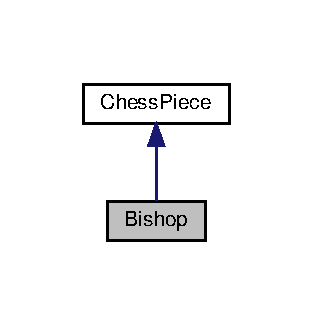
\includegraphics[width=150pt]{classBishop__inherit__graph}
\end{center}
\end{figure}


Collaboration diagram for Bishop\+:\nopagebreak
\begin{figure}[H]
\begin{center}
\leavevmode
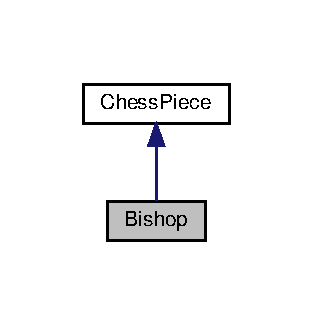
\includegraphics[width=150pt]{classBishop__coll__graph}
\end{center}
\end{figure}
\subsection*{Public Member Functions}
\begin{DoxyCompactItemize}
\item 
\hyperlink{classBishop_aaf9a04edcd25bfb97b86d6c5806e2b16}{Bishop} (\hyperlink{Enums_8h_ab87bacfdad76e61b9412d7124be44c1c}{Color} \hyperlink{classChessPiece_a8c8fc170e7c719ac2b71a93a56a38f01}{color})
\begin{DoxyCompactList}\small\item\em Constructor using \hyperlink{classChessPiece}{Chess\+Piece} constructor with \textquotesingle{}B\textquotesingle{} as an icon. \end{DoxyCompactList}\item 
bool \hyperlink{classBishop_aa9bdacc00fdb3a19035494e67240c55b}{check\+If\+Can\+Go\+To\+Position} (\hyperlink{classPosition}{Position} from\+Position, \hyperlink{classPosition}{Position} to\+Position, \hyperlink{classBoard}{Board} $\ast$board)
\begin{DoxyCompactList}\small\item\em Checks if chess piece form from\+Position can go to to\+Position. \end{DoxyCompactList}\end{DoxyCompactItemize}
\subsection*{Additional Inherited Members}


\subsection{Detailed Description}
Class responsible for handling bishop chess piece actions. 

\subsection{Constructor \& Destructor Documentation}
\mbox{\Hypertarget{classBishop_aaf9a04edcd25bfb97b86d6c5806e2b16}\label{classBishop_aaf9a04edcd25bfb97b86d6c5806e2b16}} 
\index{Bishop@{Bishop}!Bishop@{Bishop}}
\index{Bishop@{Bishop}!Bishop@{Bishop}}
\subsubsection{\texorpdfstring{Bishop()}{Bishop()}}
{\footnotesize\ttfamily Bishop\+::\+Bishop (\begin{DoxyParamCaption}\item[{\hyperlink{Enums_8h_ab87bacfdad76e61b9412d7124be44c1c}{Color}}]{color }\end{DoxyParamCaption})\hspace{0.3cm}{\ttfamily [inline]}}



Constructor using \hyperlink{classChessPiece}{Chess\+Piece} constructor with \textquotesingle{}B\textquotesingle{} as an icon. 


\begin{DoxyParams}{Parameters}
{\em color} & \\
\hline
\end{DoxyParams}
Here is the call graph for this function\+:
\nopagebreak
\begin{figure}[H]
\begin{center}
\leavevmode
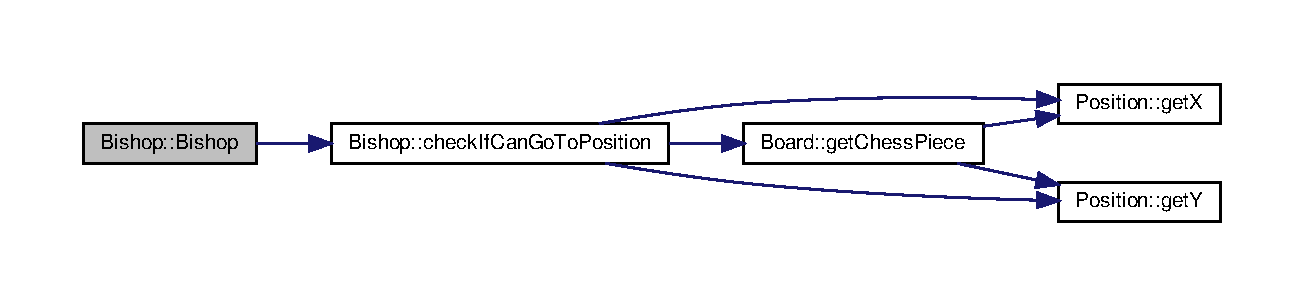
\includegraphics[width=350pt]{classBishop_aaf9a04edcd25bfb97b86d6c5806e2b16_cgraph}
\end{center}
\end{figure}


\subsection{Member Function Documentation}
\mbox{\Hypertarget{classBishop_aa9bdacc00fdb3a19035494e67240c55b}\label{classBishop_aa9bdacc00fdb3a19035494e67240c55b}} 
\index{Bishop@{Bishop}!check\+If\+Can\+Go\+To\+Position@{check\+If\+Can\+Go\+To\+Position}}
\index{check\+If\+Can\+Go\+To\+Position@{check\+If\+Can\+Go\+To\+Position}!Bishop@{Bishop}}
\subsubsection{\texorpdfstring{check\+If\+Can\+Go\+To\+Position()}{checkIfCanGoToPosition()}}
{\footnotesize\ttfamily bool Bishop\+::check\+If\+Can\+Go\+To\+Position (\begin{DoxyParamCaption}\item[{\hyperlink{classPosition}{Position}}]{from\+Position,  }\item[{\hyperlink{classPosition}{Position}}]{to\+Position,  }\item[{\hyperlink{classBoard}{Board} $\ast$}]{board }\end{DoxyParamCaption})\hspace{0.3cm}{\ttfamily [virtual]}}



Checks if chess piece form from\+Position can go to to\+Position. 


\begin{DoxyParams}{Parameters}
{\em from\+Position} & \\
\hline
{\em to\+Position} & \\
\hline
{\em board} & \\
\hline
\end{DoxyParams}
\begin{DoxyReturn}{Returns}
can\+Go 
\end{DoxyReturn}


Implements \hyperlink{classChessPiece_a90119a7c3c74ed9f967c398b8a7d7a98}{Chess\+Piece}.

Here is the call graph for this function\+:
\nopagebreak
\begin{figure}[H]
\begin{center}
\leavevmode
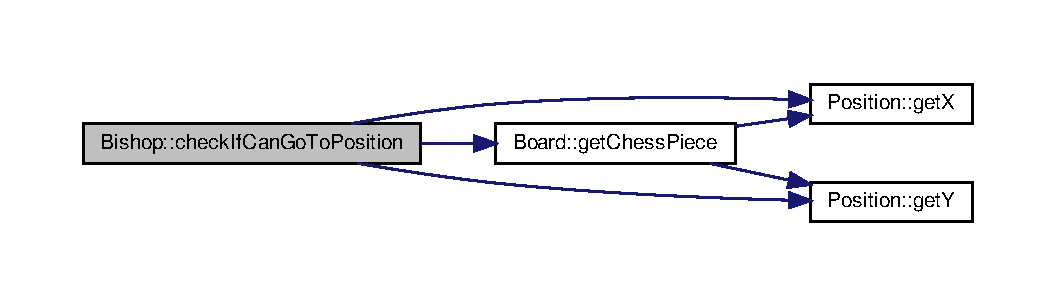
\includegraphics[width=350pt]{classBishop_aa9bdacc00fdb3a19035494e67240c55b_cgraph}
\end{center}
\end{figure}


The documentation for this class was generated from the following files\+:\begin{DoxyCompactItemize}
\item 
include/\hyperlink{Bishop_8h}{Bishop.\+h}\item 
src/\hyperlink{Bishop_8cpp}{Bishop.\+cpp}\end{DoxyCompactItemize}

\hypertarget{classBoard}{}\section{Board Class Reference}
\label{classBoard}\index{Board@{Board}}


Class responsible for handling board and board actions.  




{\ttfamily \#include $<$Board.\+h$>$}

\subsection*{Public Member Functions}
\begin{DoxyCompactItemize}
\item 
void \hyperlink{classBoard_a10531cbaada84808632ae9933c9f1306}{remove\+Chess\+Piece} (\hyperlink{classPosition}{Position} position)
\begin{DoxyCompactList}\small\item\em Removes chess piece from board. \end{DoxyCompactList}\item 
void \hyperlink{classBoard_aafb3a9f7f623360f66532e2f5fea0c2f}{set\+Chess\+Piece} (\hyperlink{classChessPiece}{Chess\+Piece} $\ast$chess\+Piece, \hyperlink{classPosition}{Position} position)
\begin{DoxyCompactList}\small\item\em Sets position on board to chess\+Piece. \end{DoxyCompactList}\item 
\hyperlink{classChessPiece}{Chess\+Piece} $\ast$ \hyperlink{classBoard_aa9344089fc229e9dcc23e58405af14d9}{get\+Chess\+Piece} (\hyperlink{classPosition}{Position} position)
\begin{DoxyCompactList}\small\item\em Returns chess piece form position. \end{DoxyCompactList}\item 
std\+::string \hyperlink{classBoard_a2cf2b2f6adc453bc3b086c9f10c77e11}{to\+String} ()
\begin{DoxyCompactList}\small\item\em Returns board converted to tidy string. \end{DoxyCompactList}\end{DoxyCompactItemize}


\subsection{Detailed Description}
Class responsible for handling board and board actions. 

\subsection{Member Function Documentation}
\mbox{\Hypertarget{classBoard_aa9344089fc229e9dcc23e58405af14d9}\label{classBoard_aa9344089fc229e9dcc23e58405af14d9}} 
\index{Board@{Board}!get\+Chess\+Piece@{get\+Chess\+Piece}}
\index{get\+Chess\+Piece@{get\+Chess\+Piece}!Board@{Board}}
\subsubsection{\texorpdfstring{get\+Chess\+Piece()}{getChessPiece()}}
{\footnotesize\ttfamily \hyperlink{classChessPiece}{Chess\+Piece} $\ast$ Board\+::get\+Chess\+Piece (\begin{DoxyParamCaption}\item[{\hyperlink{classPosition}{Position}}]{position }\end{DoxyParamCaption})}



Returns chess piece form position. 


\begin{DoxyParams}{Parameters}
{\em position} & \\
\hline
\end{DoxyParams}
\begin{DoxyReturn}{Returns}

\end{DoxyReturn}
Here is the call graph for this function\+:\nopagebreak
\begin{figure}[H]
\begin{center}
\leavevmode
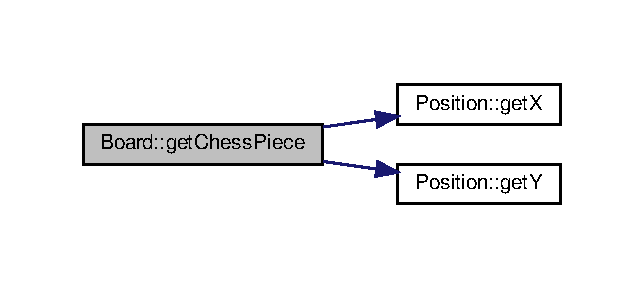
\includegraphics[width=309pt]{classBoard_aa9344089fc229e9dcc23e58405af14d9_cgraph}
\end{center}
\end{figure}
\mbox{\Hypertarget{classBoard_a10531cbaada84808632ae9933c9f1306}\label{classBoard_a10531cbaada84808632ae9933c9f1306}} 
\index{Board@{Board}!remove\+Chess\+Piece@{remove\+Chess\+Piece}}
\index{remove\+Chess\+Piece@{remove\+Chess\+Piece}!Board@{Board}}
\subsubsection{\texorpdfstring{remove\+Chess\+Piece()}{removeChessPiece()}}
{\footnotesize\ttfamily void Board\+::remove\+Chess\+Piece (\begin{DoxyParamCaption}\item[{\hyperlink{classPosition}{Position}}]{position }\end{DoxyParamCaption})}



Removes chess piece from board. 

Changes to nullptr in array.


\begin{DoxyParams}{Parameters}
{\em position} & \\
\hline
\end{DoxyParams}
Here is the call graph for this function\+:
\nopagebreak
\begin{figure}[H]
\begin{center}
\leavevmode
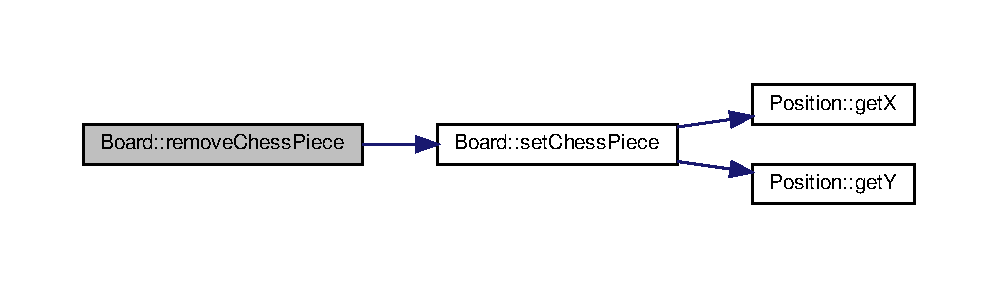
\includegraphics[width=350pt]{classBoard_a10531cbaada84808632ae9933c9f1306_cgraph}
\end{center}
\end{figure}
\mbox{\Hypertarget{classBoard_aafb3a9f7f623360f66532e2f5fea0c2f}\label{classBoard_aafb3a9f7f623360f66532e2f5fea0c2f}} 
\index{Board@{Board}!set\+Chess\+Piece@{set\+Chess\+Piece}}
\index{set\+Chess\+Piece@{set\+Chess\+Piece}!Board@{Board}}
\subsubsection{\texorpdfstring{set\+Chess\+Piece()}{setChessPiece()}}
{\footnotesize\ttfamily void Board\+::set\+Chess\+Piece (\begin{DoxyParamCaption}\item[{\hyperlink{classChessPiece}{Chess\+Piece} $\ast$}]{chess\+Piece,  }\item[{\hyperlink{classPosition}{Position}}]{position }\end{DoxyParamCaption})}



Sets position on board to chess\+Piece. 


\begin{DoxyParams}{Parameters}
{\em chess\+Piece} & \\
\hline
{\em position} & \\
\hline
\end{DoxyParams}
Here is the call graph for this function\+:\nopagebreak
\begin{figure}[H]
\begin{center}
\leavevmode
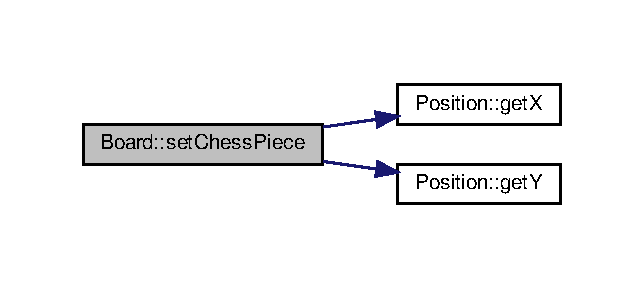
\includegraphics[width=309pt]{classBoard_aafb3a9f7f623360f66532e2f5fea0c2f_cgraph}
\end{center}
\end{figure}
\mbox{\Hypertarget{classBoard_a2cf2b2f6adc453bc3b086c9f10c77e11}\label{classBoard_a2cf2b2f6adc453bc3b086c9f10c77e11}} 
\index{Board@{Board}!to\+String@{to\+String}}
\index{to\+String@{to\+String}!Board@{Board}}
\subsubsection{\texorpdfstring{to\+String()}{toString()}}
{\footnotesize\ttfamily std\+::string Board\+::to\+String (\begin{DoxyParamCaption}{ }\end{DoxyParamCaption})}



Returns board converted to tidy string. 

\begin{DoxyReturn}{Returns}

\end{DoxyReturn}


The documentation for this class was generated from the following files\+:\begin{DoxyCompactItemize}
\item 
include/\hyperlink{Board_8h}{Board.\+h}\item 
src/\hyperlink{Board_8cpp}{Board.\+cpp}\end{DoxyCompactItemize}

\hypertarget{classChessPiece}{}\section{Chess\+Piece Class Reference}
\label{classChessPiece}\index{Chess\+Piece@{Chess\+Piece}}


Class responsible for basic chess piece actions.  




{\ttfamily \#include $<$Chess\+Piece.\+h$>$}



Inheritance diagram for Chess\+Piece\+:\nopagebreak
\begin{figure}[H]
\begin{center}
\leavevmode
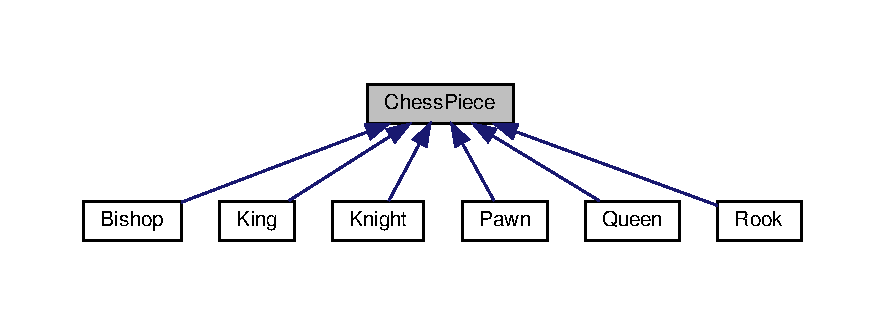
\includegraphics[width=350pt]{classChessPiece__inherit__graph}
\end{center}
\end{figure}
\subsection*{Public Member Functions}
\begin{DoxyCompactItemize}
\item 
\hyperlink{classChessPiece_a38c44e06d7bf1b0f96d27886ca5d389f}{Chess\+Piece} (\hyperlink{Enums_8h_ab87bacfdad76e61b9412d7124be44c1c}{Color} \hyperlink{classChessPiece_a8c8fc170e7c719ac2b71a93a56a38f01}{color}, char \hyperlink{classChessPiece_ad32540487648131ed69e63f46f787d08}{icon})
\begin{DoxyCompactList}\small\item\em Constructor. \end{DoxyCompactList}\item 
virtual bool \hyperlink{classChessPiece_a90119a7c3c74ed9f967c398b8a7d7a98}{check\+If\+Can\+Go\+To\+Position} (\hyperlink{classPosition}{Position} form\+Position, \hyperlink{classPosition}{Position} to\+Position, \hyperlink{classBoard}{Board} $\ast$board)=0
\begin{DoxyCompactList}\small\item\em Checks if chess piece form from\+Position can go to to\+Position. \end{DoxyCompactList}\item 
\hyperlink{Enums_8h_ab87bacfdad76e61b9412d7124be44c1c}{Color} \hyperlink{classChessPiece_a99f599eac60792290e3bcb3bea1e0970}{get\+Color} ()
\begin{DoxyCompactList}\small\item\em Reurns color of the chess piece. \end{DoxyCompactList}\item 
char \hyperlink{classChessPiece_aee72609f866105f5676e007887877b7c}{get\+Icon} ()
\begin{DoxyCompactList}\small\item\em Returns icon of the chess piece. \end{DoxyCompactList}\end{DoxyCompactItemize}
\subsection*{Protected Attributes}
\begin{DoxyCompactItemize}
\item 
\mbox{\Hypertarget{classChessPiece_a8c8fc170e7c719ac2b71a93a56a38f01}\label{classChessPiece_a8c8fc170e7c719ac2b71a93a56a38f01}} 
\hyperlink{Enums_8h_ab87bacfdad76e61b9412d7124be44c1c}{Color} \hyperlink{classChessPiece_a8c8fc170e7c719ac2b71a93a56a38f01}{color}
\begin{DoxyCompactList}\small\item\em Color of the chess piece. \end{DoxyCompactList}\item 
\mbox{\Hypertarget{classChessPiece_ad32540487648131ed69e63f46f787d08}\label{classChessPiece_ad32540487648131ed69e63f46f787d08}} 
char \hyperlink{classChessPiece_ad32540487648131ed69e63f46f787d08}{icon}
\begin{DoxyCompactList}\small\item\em Char which will be show when displaying chess piece. \end{DoxyCompactList}\end{DoxyCompactItemize}


\subsection{Detailed Description}
Class responsible for basic chess piece actions. 

\subsection{Constructor \& Destructor Documentation}
\mbox{\Hypertarget{classChessPiece_a38c44e06d7bf1b0f96d27886ca5d389f}\label{classChessPiece_a38c44e06d7bf1b0f96d27886ca5d389f}} 
\index{Chess\+Piece@{Chess\+Piece}!Chess\+Piece@{Chess\+Piece}}
\index{Chess\+Piece@{Chess\+Piece}!Chess\+Piece@{Chess\+Piece}}
\subsubsection{\texorpdfstring{Chess\+Piece()}{ChessPiece()}}
{\footnotesize\ttfamily Chess\+Piece\+::\+Chess\+Piece (\begin{DoxyParamCaption}\item[{\hyperlink{Enums_8h_ab87bacfdad76e61b9412d7124be44c1c}{Color}}]{color,  }\item[{char}]{icon }\end{DoxyParamCaption})}



Constructor. 


\begin{DoxyParams}{Parameters}
{\em color} & \\
\hline
{\em icon} & \\
\hline
\end{DoxyParams}


\subsection{Member Function Documentation}
\mbox{\Hypertarget{classChessPiece_a90119a7c3c74ed9f967c398b8a7d7a98}\label{classChessPiece_a90119a7c3c74ed9f967c398b8a7d7a98}} 
\index{Chess\+Piece@{Chess\+Piece}!check\+If\+Can\+Go\+To\+Position@{check\+If\+Can\+Go\+To\+Position}}
\index{check\+If\+Can\+Go\+To\+Position@{check\+If\+Can\+Go\+To\+Position}!Chess\+Piece@{Chess\+Piece}}
\subsubsection{\texorpdfstring{check\+If\+Can\+Go\+To\+Position()}{checkIfCanGoToPosition()}}
{\footnotesize\ttfamily virtual bool Chess\+Piece\+::check\+If\+Can\+Go\+To\+Position (\begin{DoxyParamCaption}\item[{\hyperlink{classPosition}{Position}}]{form\+Position,  }\item[{\hyperlink{classPosition}{Position}}]{to\+Position,  }\item[{\hyperlink{classBoard}{Board} $\ast$}]{board }\end{DoxyParamCaption})\hspace{0.3cm}{\ttfamily [pure virtual]}}



Checks if chess piece form from\+Position can go to to\+Position. 


\begin{DoxyParams}{Parameters}
{\em form\+Position} & \\
\hline
{\em to\+Position} & \\
\hline
{\em board} & \\
\hline
\end{DoxyParams}
\begin{DoxyReturn}{Returns}

\end{DoxyReturn}


Implemented in \hyperlink{classQueen_a504eb0f657c4ae6acbf54ef8ab4c5cf9}{Queen}, \hyperlink{classPawn_a30abb1fc67dffcd5f9ae104baf3e27ac}{Pawn}, \hyperlink{classBishop_aa9bdacc00fdb3a19035494e67240c55b}{Bishop}, \hyperlink{classKing_ab9e40ed32cfc93fec76a831d2087fa78}{King}, \hyperlink{classRook_aad67c9012197bf285cf6a27861fbcb06}{Rook}, and \hyperlink{classKnight_a8aaec0101a97586e884332bf15787319}{Knight}.

\mbox{\Hypertarget{classChessPiece_a99f599eac60792290e3bcb3bea1e0970}\label{classChessPiece_a99f599eac60792290e3bcb3bea1e0970}} 
\index{Chess\+Piece@{Chess\+Piece}!get\+Color@{get\+Color}}
\index{get\+Color@{get\+Color}!Chess\+Piece@{Chess\+Piece}}
\subsubsection{\texorpdfstring{get\+Color()}{getColor()}}
{\footnotesize\ttfamily \hyperlink{Enums_8h_ab87bacfdad76e61b9412d7124be44c1c}{Color} Chess\+Piece\+::get\+Color (\begin{DoxyParamCaption}{ }\end{DoxyParamCaption})}



Reurns color of the chess piece. 

\begin{DoxyReturn}{Returns}

\end{DoxyReturn}
\mbox{\Hypertarget{classChessPiece_aee72609f866105f5676e007887877b7c}\label{classChessPiece_aee72609f866105f5676e007887877b7c}} 
\index{Chess\+Piece@{Chess\+Piece}!get\+Icon@{get\+Icon}}
\index{get\+Icon@{get\+Icon}!Chess\+Piece@{Chess\+Piece}}
\subsubsection{\texorpdfstring{get\+Icon()}{getIcon()}}
{\footnotesize\ttfamily char Chess\+Piece\+::get\+Icon (\begin{DoxyParamCaption}{ }\end{DoxyParamCaption})}



Returns icon of the chess piece. 

\begin{DoxyReturn}{Returns}

\end{DoxyReturn}


The documentation for this class was generated from the following files\+:\begin{DoxyCompactItemize}
\item 
include/\hyperlink{ChessPiece_8h}{Chess\+Piece.\+h}\item 
src/\hyperlink{ChessPiece_8cpp}{Chess\+Piece.\+cpp}\end{DoxyCompactItemize}

\hypertarget{classGameInterface}{}\section{Game\+Interface Class Reference}
\label{classGameInterface}\index{Game\+Interface@{Game\+Interface}}


Class responsible for user interface.  




{\ttfamily \#include $<$Game\+Interface.\+h$>$}

\subsection*{Public Member Functions}
\begin{DoxyCompactItemize}
\item 
\hyperlink{classGameInterface_acb731c8610dcb344635269863fc1c36d}{Game\+Interface} (\hyperlink{classGameManager}{Game\+Manager} $\ast$game\+Manager)
\begin{DoxyCompactList}\small\item\em Constructor. \end{DoxyCompactList}\item 
\mbox{\Hypertarget{classGameInterface_af61f3f8a7da96ae1cbad04b6f400ab0a}\label{classGameInterface_af61f3f8a7da96ae1cbad04b6f400ab0a}} 
\hyperlink{classGameInterface_af61f3f8a7da96ae1cbad04b6f400ab0a}{$\sim$\+Game\+Interface} ()
\begin{DoxyCompactList}\small\item\em Destructor. \end{DoxyCompactList}\item 
\mbox{\Hypertarget{classGameInterface_afa5ac9d56e2578c26acbf528946827f3}\label{classGameInterface_afa5ac9d56e2578c26acbf528946827f3}} 
void \hyperlink{classGameInterface_afa5ac9d56e2578c26acbf528946827f3}{play\+Game} ()
\begin{DoxyCompactList}\small\item\em Starts game loop. \end{DoxyCompactList}\end{DoxyCompactItemize}


\subsection{Detailed Description}
Class responsible for user interface. 

\subsection{Constructor \& Destructor Documentation}
\mbox{\Hypertarget{classGameInterface_acb731c8610dcb344635269863fc1c36d}\label{classGameInterface_acb731c8610dcb344635269863fc1c36d}} 
\index{Game\+Interface@{Game\+Interface}!Game\+Interface@{Game\+Interface}}
\index{Game\+Interface@{Game\+Interface}!Game\+Interface@{Game\+Interface}}
\subsubsection{\texorpdfstring{Game\+Interface()}{GameInterface()}}
{\footnotesize\ttfamily Game\+Interface\+::\+Game\+Interface (\begin{DoxyParamCaption}\item[{\hyperlink{classGameManager}{Game\+Manager} $\ast$}]{game\+Manager }\end{DoxyParamCaption})}



Constructor. 


\begin{DoxyParams}{Parameters}
{\em game\+Manager} & \\
\hline
\end{DoxyParams}


The documentation for this class was generated from the following files\+:\begin{DoxyCompactItemize}
\item 
include/\hyperlink{GameInterface_8h}{Game\+Interface.\+h}\item 
src/\hyperlink{GameInterface_8cpp}{Game\+Interface.\+cpp}\end{DoxyCompactItemize}

\hypertarget{classGameManager}{}\section{Game\+Manager Class Reference}
\label{classGameManager}\index{Game\+Manager@{Game\+Manager}}


Class responsible for managing game logic.  




{\ttfamily \#include $<$Game\+Manager.\+h$>$}

\subsection*{Public Member Functions}
\begin{DoxyCompactItemize}
\item 
\hyperlink{classGameManager_a79d810aa82d8987c1cdb0e67a7f361fb}{Game\+Manager} (\hyperlink{classBoard}{Board} $\ast$board)
\begin{DoxyCompactList}\small\item\em Constructor. \end{DoxyCompactList}\item 
bool \hyperlink{classGameManager_a115bc92a76d5a500667601ede0becb07}{make\+Move} (\hyperlink{classPosition}{Position} chess\+Piece\+To\+Move\+Position, \hyperlink{classPosition}{Position} position\+To\+Move\+To, \hyperlink{Enums_8h_ab87bacfdad76e61b9412d7124be44c1c}{Color} player\+Moving\+Color)
\begin{DoxyCompactList}\small\item\em Check and moves if chess piece from chess\+Piece\+To\+Move\+Position can go to position\+To\+Move\+To, if current player is player\+Moving\+Color. \end{DoxyCompactList}\item 
std\+::string \hyperlink{classGameManager_a882cb4b776ef8d0e6912c175d746fcdd}{board\+To\+String} ()
\begin{DoxyCompactList}\small\item\em Returns board in tidy string. \end{DoxyCompactList}\end{DoxyCompactItemize}


\subsection{Detailed Description}
Class responsible for managing game logic. 

\subsection{Constructor \& Destructor Documentation}
\mbox{\Hypertarget{classGameManager_a79d810aa82d8987c1cdb0e67a7f361fb}\label{classGameManager_a79d810aa82d8987c1cdb0e67a7f361fb}} 
\index{Game\+Manager@{Game\+Manager}!Game\+Manager@{Game\+Manager}}
\index{Game\+Manager@{Game\+Manager}!Game\+Manager@{Game\+Manager}}
\subsubsection{\texorpdfstring{Game\+Manager()}{GameManager()}}
{\footnotesize\ttfamily Game\+Manager\+::\+Game\+Manager (\begin{DoxyParamCaption}\item[{\hyperlink{classBoard}{Board} $\ast$}]{board }\end{DoxyParamCaption})}



Constructor. 


\begin{DoxyParams}{Parameters}
{\em board} & \\
\hline
\end{DoxyParams}


\subsection{Member Function Documentation}
\mbox{\Hypertarget{classGameManager_a882cb4b776ef8d0e6912c175d746fcdd}\label{classGameManager_a882cb4b776ef8d0e6912c175d746fcdd}} 
\index{Game\+Manager@{Game\+Manager}!board\+To\+String@{board\+To\+String}}
\index{board\+To\+String@{board\+To\+String}!Game\+Manager@{Game\+Manager}}
\subsubsection{\texorpdfstring{board\+To\+String()}{boardToString()}}
{\footnotesize\ttfamily std\+::string Game\+Manager\+::board\+To\+String (\begin{DoxyParamCaption}{ }\end{DoxyParamCaption})}



Returns board in tidy string. 

\begin{DoxyReturn}{Returns}

\end{DoxyReturn}
Here is the call graph for this function\+:
\nopagebreak
\begin{figure}[H]
\begin{center}
\leavevmode
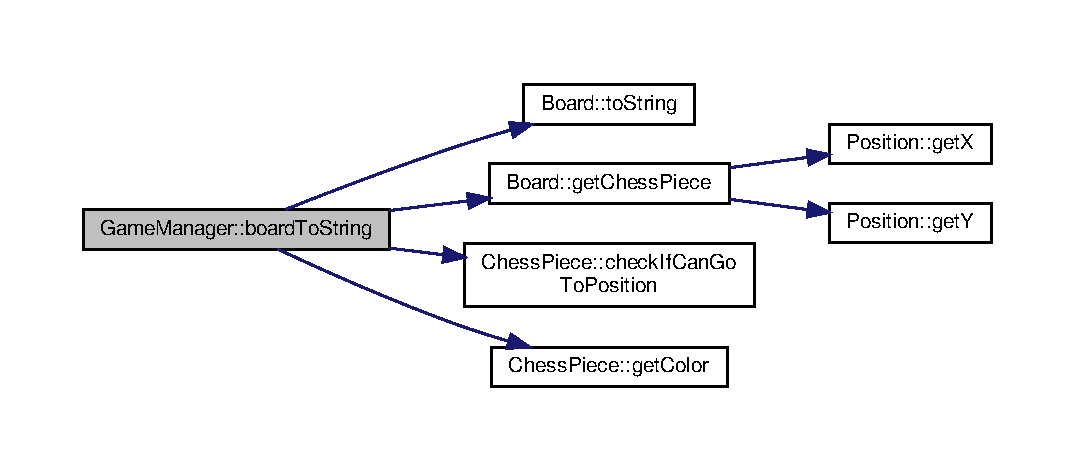
\includegraphics[width=350pt]{classGameManager_a882cb4b776ef8d0e6912c175d746fcdd_cgraph}
\end{center}
\end{figure}
\mbox{\Hypertarget{classGameManager_a115bc92a76d5a500667601ede0becb07}\label{classGameManager_a115bc92a76d5a500667601ede0becb07}} 
\index{Game\+Manager@{Game\+Manager}!make\+Move@{make\+Move}}
\index{make\+Move@{make\+Move}!Game\+Manager@{Game\+Manager}}
\subsubsection{\texorpdfstring{make\+Move()}{makeMove()}}
{\footnotesize\ttfamily bool Game\+Manager\+::make\+Move (\begin{DoxyParamCaption}\item[{\hyperlink{classPosition}{Position}}]{chess\+Piece\+To\+Move\+Position,  }\item[{\hyperlink{classPosition}{Position}}]{position\+To\+Move\+To,  }\item[{\hyperlink{Enums_8h_ab87bacfdad76e61b9412d7124be44c1c}{Color}}]{player\+Moving\+Color }\end{DoxyParamCaption})}



Check and moves if chess piece from chess\+Piece\+To\+Move\+Position can go to position\+To\+Move\+To, if current player is player\+Moving\+Color. 


\begin{DoxyParams}{Parameters}
{\em chess\+Piece\+To\+Move\+Position} & \\
\hline
{\em position\+To\+Move\+To} & \\
\hline
{\em player\+Moving\+Color} & \\
\hline
\end{DoxyParams}
\begin{DoxyReturn}{Returns}
move\+Made 
\end{DoxyReturn}
Here is the call graph for this function\+:\nopagebreak
\begin{figure}[H]
\begin{center}
\leavevmode
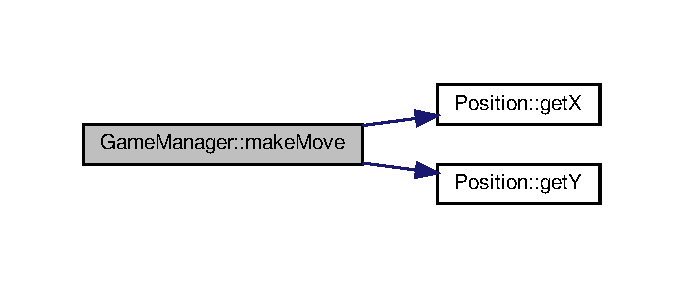
\includegraphics[width=328pt]{classGameManager_a115bc92a76d5a500667601ede0becb07_cgraph}
\end{center}
\end{figure}


The documentation for this class was generated from the following files\+:\begin{DoxyCompactItemize}
\item 
include/\hyperlink{GameManager_8h}{Game\+Manager.\+h}\item 
src/\hyperlink{GameManager_8cpp}{Game\+Manager.\+cpp}\end{DoxyCompactItemize}

\hypertarget{classKing}{}\section{King Class Reference}
\label{classKing}\index{King@{King}}


Class responsible for king chess piece actions.  




{\ttfamily \#include $<$King.\+h$>$}



Inheritance diagram for King\+:\nopagebreak
\begin{figure}[H]
\begin{center}
\leavevmode
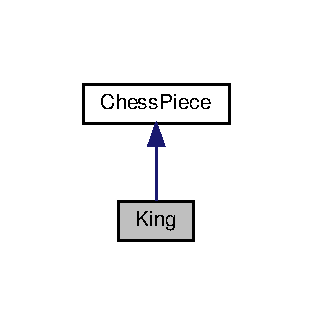
\includegraphics[width=150pt]{classKing__inherit__graph}
\end{center}
\end{figure}


Collaboration diagram for King\+:\nopagebreak
\begin{figure}[H]
\begin{center}
\leavevmode
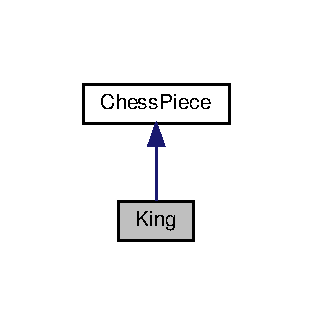
\includegraphics[width=150pt]{classKing__coll__graph}
\end{center}
\end{figure}
\subsection*{Public Member Functions}
\begin{DoxyCompactItemize}
\item 
\hyperlink{classKing_a39c7835e28a746800a290c3fb6501c92}{King} (\hyperlink{Enums_8h_ab87bacfdad76e61b9412d7124be44c1c}{Color} \hyperlink{classChessPiece_a8c8fc170e7c719ac2b71a93a56a38f01}{color})
\begin{DoxyCompactList}\small\item\em Constructor using \hyperlink{classChessPiece}{Chess\+Piece} constructor and \textquotesingle{}K" as icon. \end{DoxyCompactList}\item 
bool \hyperlink{classKing_ab9e40ed32cfc93fec76a831d2087fa78}{check\+If\+Can\+Go\+To\+Position} (\hyperlink{classPosition}{Position} from\+Position, \hyperlink{classPosition}{Position} to\+Position, \hyperlink{classBoard}{Board} $\ast$board)
\begin{DoxyCompactList}\small\item\em Checks if king form from\+Position can go to to\+Position. \end{DoxyCompactList}\end{DoxyCompactItemize}
\subsection*{Additional Inherited Members}


\subsection{Detailed Description}
Class responsible for king chess piece actions. 

\subsection{Constructor \& Destructor Documentation}
\mbox{\Hypertarget{classKing_a39c7835e28a746800a290c3fb6501c92}\label{classKing_a39c7835e28a746800a290c3fb6501c92}} 
\index{King@{King}!King@{King}}
\index{King@{King}!King@{King}}
\subsubsection{\texorpdfstring{King()}{King()}}
{\footnotesize\ttfamily King\+::\+King (\begin{DoxyParamCaption}\item[{\hyperlink{Enums_8h_ab87bacfdad76e61b9412d7124be44c1c}{Color}}]{color }\end{DoxyParamCaption})\hspace{0.3cm}{\ttfamily [inline]}}



Constructor using \hyperlink{classChessPiece}{Chess\+Piece} constructor and \textquotesingle{}K" as icon. 


\begin{DoxyParams}{Parameters}
{\em color} & \\
\hline
\end{DoxyParams}
Here is the call graph for this function\+:
\nopagebreak
\begin{figure}[H]
\begin{center}
\leavevmode
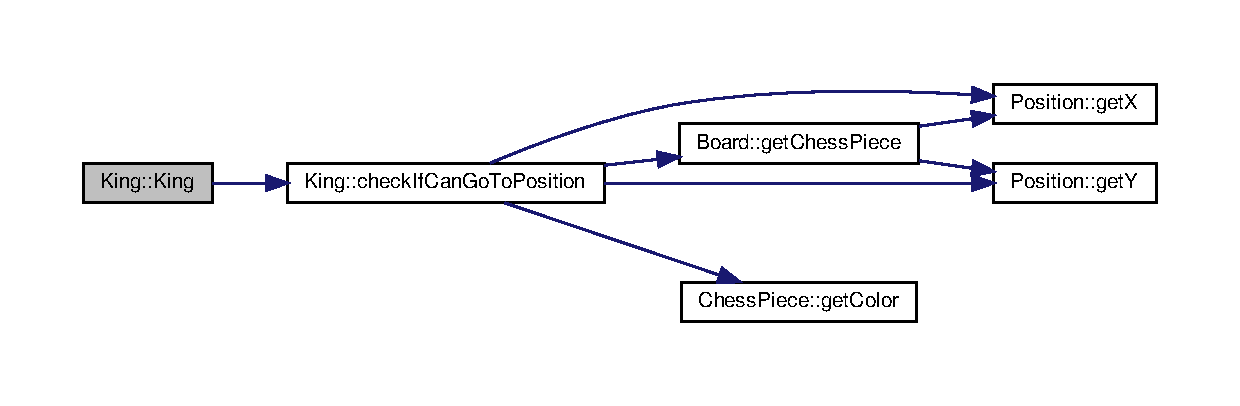
\includegraphics[width=350pt]{classKing_a39c7835e28a746800a290c3fb6501c92_cgraph}
\end{center}
\end{figure}


\subsection{Member Function Documentation}
\mbox{\Hypertarget{classKing_ab9e40ed32cfc93fec76a831d2087fa78}\label{classKing_ab9e40ed32cfc93fec76a831d2087fa78}} 
\index{King@{King}!check\+If\+Can\+Go\+To\+Position@{check\+If\+Can\+Go\+To\+Position}}
\index{check\+If\+Can\+Go\+To\+Position@{check\+If\+Can\+Go\+To\+Position}!King@{King}}
\subsubsection{\texorpdfstring{check\+If\+Can\+Go\+To\+Position()}{checkIfCanGoToPosition()}}
{\footnotesize\ttfamily bool King\+::check\+If\+Can\+Go\+To\+Position (\begin{DoxyParamCaption}\item[{\hyperlink{classPosition}{Position}}]{from\+Position,  }\item[{\hyperlink{classPosition}{Position}}]{to\+Position,  }\item[{\hyperlink{classBoard}{Board} $\ast$}]{board }\end{DoxyParamCaption})\hspace{0.3cm}{\ttfamily [virtual]}}



Checks if king form from\+Position can go to to\+Position. 


\begin{DoxyParams}{Parameters}
{\em from\+Position} & \\
\hline
{\em to\+Position} & \\
\hline
{\em board} & \\
\hline
\end{DoxyParams}
\begin{DoxyReturn}{Returns}
can\+Move 
\end{DoxyReturn}


Implements \hyperlink{classChessPiece_a90119a7c3c74ed9f967c398b8a7d7a98}{Chess\+Piece}.

Here is the call graph for this function\+:
\nopagebreak
\begin{figure}[H]
\begin{center}
\leavevmode
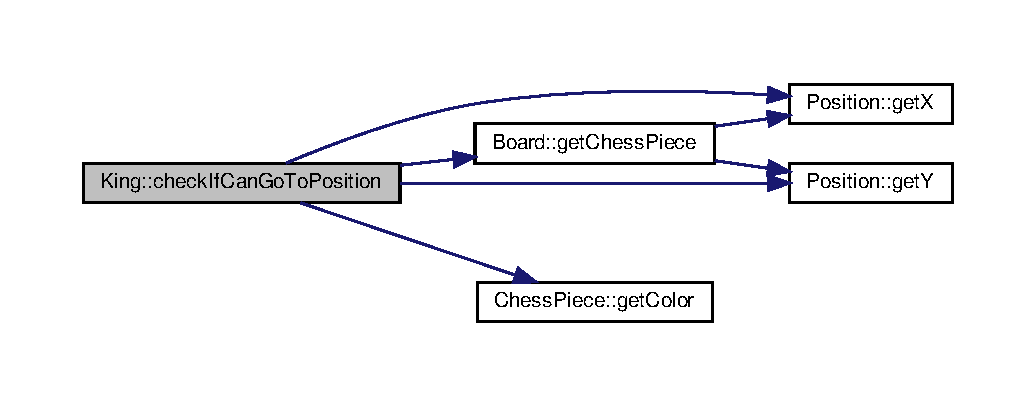
\includegraphics[width=350pt]{classKing_ab9e40ed32cfc93fec76a831d2087fa78_cgraph}
\end{center}
\end{figure}


The documentation for this class was generated from the following files\+:\begin{DoxyCompactItemize}
\item 
include/\hyperlink{King_8h}{King.\+h}\item 
src/\hyperlink{King_8cpp}{King.\+cpp}\end{DoxyCompactItemize}

\hypertarget{classKnight}{}\section{Knight Class Reference}
\label{classKnight}\index{Knight@{Knight}}


Class responsible for knight chess piece actions.  




{\ttfamily \#include $<$Knight.\+h$>$}



Inheritance diagram for Knight\+:\nopagebreak
\begin{figure}[H]
\begin{center}
\leavevmode
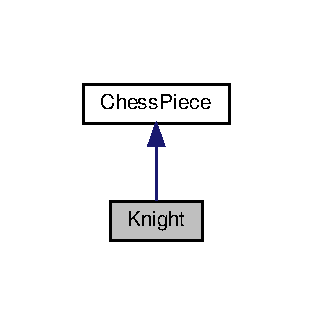
\includegraphics[width=150pt]{classKnight__inherit__graph}
\end{center}
\end{figure}


Collaboration diagram for Knight\+:\nopagebreak
\begin{figure}[H]
\begin{center}
\leavevmode
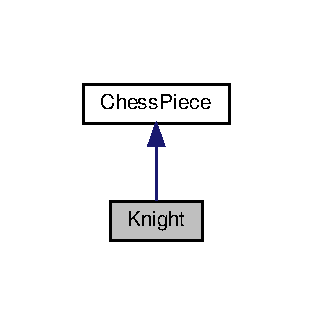
\includegraphics[width=150pt]{classKnight__coll__graph}
\end{center}
\end{figure}
\subsection*{Public Member Functions}
\begin{DoxyCompactItemize}
\item 
\hyperlink{classKnight_ac26ef96049f2e732b0adbc829b66939d}{Knight} (\hyperlink{Enums_8h_ab87bacfdad76e61b9412d7124be44c1c}{Color} \hyperlink{classChessPiece_a8c8fc170e7c719ac2b71a93a56a38f01}{color})
\begin{DoxyCompactList}\small\item\em Constructor using \hyperlink{classChessPiece}{Chess\+Piece} constructor and \textquotesingle{}S\textquotesingle{} as icon. \end{DoxyCompactList}\item 
bool \hyperlink{classKnight_a8aaec0101a97586e884332bf15787319}{check\+If\+Can\+Go\+To\+Position} (\hyperlink{classPosition}{Position} from\+Position, \hyperlink{classPosition}{Position} to\+Position, \hyperlink{classBoard}{Board} $\ast$board)
\begin{DoxyCompactList}\small\item\em Checks if chess piece form from\+Position can go to to\+Position . \end{DoxyCompactList}\end{DoxyCompactItemize}
\subsection*{Additional Inherited Members}


\subsection{Detailed Description}
Class responsible for knight chess piece actions. 

\subsection{Constructor \& Destructor Documentation}
\mbox{\Hypertarget{classKnight_ac26ef96049f2e732b0adbc829b66939d}\label{classKnight_ac26ef96049f2e732b0adbc829b66939d}} 
\index{Knight@{Knight}!Knight@{Knight}}
\index{Knight@{Knight}!Knight@{Knight}}
\subsubsection{\texorpdfstring{Knight()}{Knight()}}
{\footnotesize\ttfamily Knight\+::\+Knight (\begin{DoxyParamCaption}\item[{\hyperlink{Enums_8h_ab87bacfdad76e61b9412d7124be44c1c}{Color}}]{color }\end{DoxyParamCaption})\hspace{0.3cm}{\ttfamily [inline]}}



Constructor using \hyperlink{classChessPiece}{Chess\+Piece} constructor and \textquotesingle{}S\textquotesingle{} as icon. 


\begin{DoxyParams}{Parameters}
{\em color} & \\
\hline
\end{DoxyParams}
Here is the call graph for this function\+:
\nopagebreak
\begin{figure}[H]
\begin{center}
\leavevmode
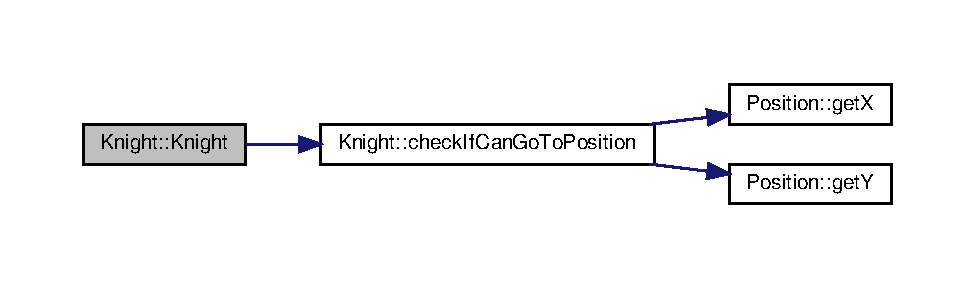
\includegraphics[width=350pt]{classKnight_ac26ef96049f2e732b0adbc829b66939d_cgraph}
\end{center}
\end{figure}


\subsection{Member Function Documentation}
\mbox{\Hypertarget{classKnight_a8aaec0101a97586e884332bf15787319}\label{classKnight_a8aaec0101a97586e884332bf15787319}} 
\index{Knight@{Knight}!check\+If\+Can\+Go\+To\+Position@{check\+If\+Can\+Go\+To\+Position}}
\index{check\+If\+Can\+Go\+To\+Position@{check\+If\+Can\+Go\+To\+Position}!Knight@{Knight}}
\subsubsection{\texorpdfstring{check\+If\+Can\+Go\+To\+Position()}{checkIfCanGoToPosition()}}
{\footnotesize\ttfamily bool Knight\+::check\+If\+Can\+Go\+To\+Position (\begin{DoxyParamCaption}\item[{\hyperlink{classPosition}{Position}}]{from\+Position,  }\item[{\hyperlink{classPosition}{Position}}]{to\+Position,  }\item[{\hyperlink{classBoard}{Board} $\ast$}]{board }\end{DoxyParamCaption})\hspace{0.3cm}{\ttfamily [virtual]}}



Checks if chess piece form from\+Position can go to to\+Position . 


\begin{DoxyParams}{Parameters}
{\em from\+Position} & \\
\hline
{\em to\+Position} & \\
\hline
{\em board} & \\
\hline
\end{DoxyParams}
\begin{DoxyReturn}{Returns}
can\+Move 
\end{DoxyReturn}


Implements \hyperlink{classChessPiece_a90119a7c3c74ed9f967c398b8a7d7a98}{Chess\+Piece}.

Here is the call graph for this function\+:\nopagebreak
\begin{figure}[H]
\begin{center}
\leavevmode
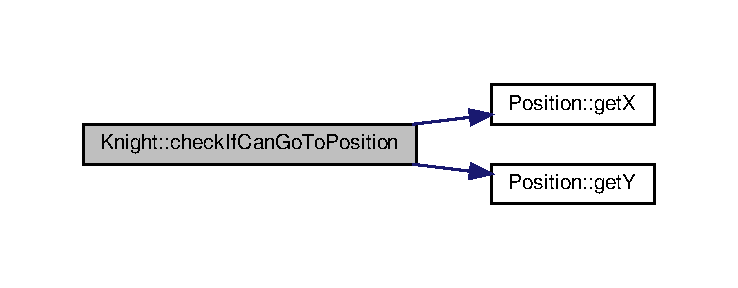
\includegraphics[width=350pt]{classKnight_a8aaec0101a97586e884332bf15787319_cgraph}
\end{center}
\end{figure}


The documentation for this class was generated from the following files\+:\begin{DoxyCompactItemize}
\item 
include/\hyperlink{Knight_8h}{Knight.\+h}\item 
src/\hyperlink{Knight_8cpp}{Knight.\+cpp}\end{DoxyCompactItemize}

\hypertarget{classPathPattern}{}\section{Path\+Pattern Class Reference}
\label{classPathPattern}\index{Path\+Pattern@{Path\+Pattern}}


Relict class.  




{\ttfamily \#include $<$Path\+Pattern.\+h$>$}

\subsection*{Public Member Functions}
\begin{DoxyCompactItemize}
\item 
\mbox{\Hypertarget{classPathPattern_aedf0fca346f2d4e00da5f6b4583239a8}\label{classPathPattern_aedf0fca346f2d4e00da5f6b4583239a8}} 
{\bfseries Path\+Pattern} (bool is\+Repetetive, \hyperlink{classPosition}{Position} end\+Position, \hyperlink{Enums_8h_a224b9163917ac32fc95a60d8c1eec3aa}{Direction} available\+Directions\mbox{[}$\,$\mbox{]})
\item 
\mbox{\Hypertarget{classPathPattern_a4bc143c302c4a1145c219deef2c703c1}\label{classPathPattern_a4bc143c302c4a1145c219deef2c703c1}} 
bool {\bfseries get\+Is\+Repetetive} ()
\item 
\mbox{\Hypertarget{classPathPattern_ae2a5b89bdc4d39c2a46bddcf9ea2c88b}\label{classPathPattern_ae2a5b89bdc4d39c2a46bddcf9ea2c88b}} 
\hyperlink{classPosition}{Position} {\bfseries get\+End\+Position} ()
\item 
\mbox{\Hypertarget{classPathPattern_abd89be9f28845abaab3d45d0a89351c1}\label{classPathPattern_abd89be9f28845abaab3d45d0a89351c1}} 
\hyperlink{Enums_8h_a224b9163917ac32fc95a60d8c1eec3aa}{Direction} {\bfseries get\+Available\+Directions} ()
\end{DoxyCompactItemize}


\subsection{Detailed Description}
Relict class. 

The documentation for this class was generated from the following file\+:\begin{DoxyCompactItemize}
\item 
include/Path\+Pattern.\+h\end{DoxyCompactItemize}

\hypertarget{classPawn}{}\section{Pawn Class Reference}
\label{classPawn}\index{Pawn@{Pawn}}


Class responsible for pawn chess piece actions.  




{\ttfamily \#include $<$Pawn.\+h$>$}



Inheritance diagram for Pawn\+:\nopagebreak
\begin{figure}[H]
\begin{center}
\leavevmode
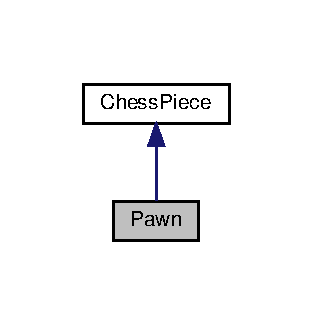
\includegraphics[width=150pt]{classPawn__inherit__graph}
\end{center}
\end{figure}


Collaboration diagram for Pawn\+:\nopagebreak
\begin{figure}[H]
\begin{center}
\leavevmode
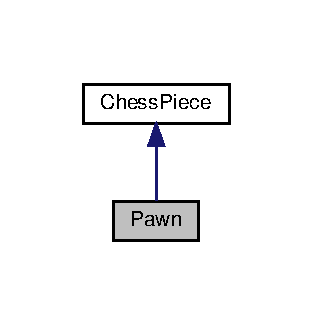
\includegraphics[width=150pt]{classPawn__coll__graph}
\end{center}
\end{figure}
\subsection*{Public Member Functions}
\begin{DoxyCompactItemize}
\item 
\hyperlink{classPawn_a3e1ac517cf828f52957f54179a455922}{Pawn} (\hyperlink{Enums_8h_ab87bacfdad76e61b9412d7124be44c1c}{Color} \hyperlink{classChessPiece_a8c8fc170e7c719ac2b71a93a56a38f01}{color})
\begin{DoxyCompactList}\small\item\em Constructor using \hyperlink{classChessPiece}{Chess\+Piece} constructor and \textquotesingle{}P\textquotesingle{} as an icon. \end{DoxyCompactList}\item 
bool \hyperlink{classPawn_a30abb1fc67dffcd5f9ae104baf3e27ac}{check\+If\+Can\+Go\+To\+Position} (\hyperlink{classPosition}{Position} from\+Position, \hyperlink{classPosition}{Position} to\+Position, \hyperlink{classBoard}{Board} $\ast$board)
\begin{DoxyCompactList}\small\item\em Checks if pawn form from\+Position can go to to\+Position. \end{DoxyCompactList}\end{DoxyCompactItemize}
\subsection*{Additional Inherited Members}


\subsection{Detailed Description}
Class responsible for pawn chess piece actions. 

\subsection{Constructor \& Destructor Documentation}
\mbox{\Hypertarget{classPawn_a3e1ac517cf828f52957f54179a455922}\label{classPawn_a3e1ac517cf828f52957f54179a455922}} 
\index{Pawn@{Pawn}!Pawn@{Pawn}}
\index{Pawn@{Pawn}!Pawn@{Pawn}}
\subsubsection{\texorpdfstring{Pawn()}{Pawn()}}
{\footnotesize\ttfamily Pawn\+::\+Pawn (\begin{DoxyParamCaption}\item[{\hyperlink{Enums_8h_ab87bacfdad76e61b9412d7124be44c1c}{Color}}]{color }\end{DoxyParamCaption})\hspace{0.3cm}{\ttfamily [inline]}}



Constructor using \hyperlink{classChessPiece}{Chess\+Piece} constructor and \textquotesingle{}P\textquotesingle{} as an icon. 


\begin{DoxyParams}{Parameters}
{\em color} & \\
\hline
\end{DoxyParams}
Here is the call graph for this function\+:
\nopagebreak
\begin{figure}[H]
\begin{center}
\leavevmode
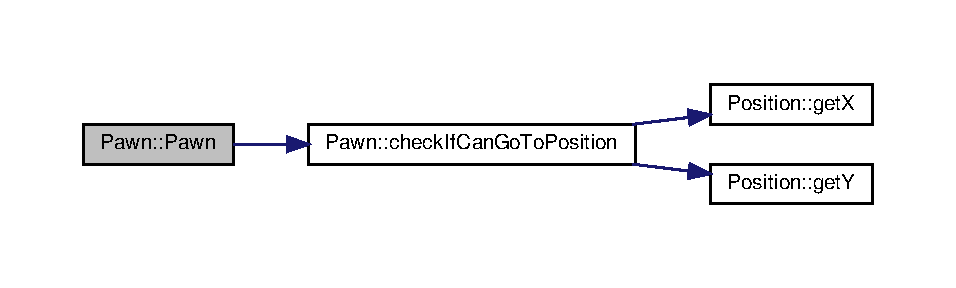
\includegraphics[width=350pt]{classPawn_a3e1ac517cf828f52957f54179a455922_cgraph}
\end{center}
\end{figure}


\subsection{Member Function Documentation}
\mbox{\Hypertarget{classPawn_a30abb1fc67dffcd5f9ae104baf3e27ac}\label{classPawn_a30abb1fc67dffcd5f9ae104baf3e27ac}} 
\index{Pawn@{Pawn}!check\+If\+Can\+Go\+To\+Position@{check\+If\+Can\+Go\+To\+Position}}
\index{check\+If\+Can\+Go\+To\+Position@{check\+If\+Can\+Go\+To\+Position}!Pawn@{Pawn}}
\subsubsection{\texorpdfstring{check\+If\+Can\+Go\+To\+Position()}{checkIfCanGoToPosition()}}
{\footnotesize\ttfamily bool Pawn\+::check\+If\+Can\+Go\+To\+Position (\begin{DoxyParamCaption}\item[{\hyperlink{classPosition}{Position}}]{from\+Position,  }\item[{\hyperlink{classPosition}{Position}}]{to\+Position,  }\item[{\hyperlink{classBoard}{Board} $\ast$}]{board }\end{DoxyParamCaption})\hspace{0.3cm}{\ttfamily [virtual]}}



Checks if pawn form from\+Position can go to to\+Position. 


\begin{DoxyParams}{Parameters}
{\em from\+Position} & \\
\hline
{\em to\+Position} & \\
\hline
{\em board} & \\
\hline
\end{DoxyParams}
\begin{DoxyReturn}{Returns}

\end{DoxyReturn}


Implements \hyperlink{classChessPiece_a90119a7c3c74ed9f967c398b8a7d7a98}{Chess\+Piece}.

Here is the call graph for this function\+:\nopagebreak
\begin{figure}[H]
\begin{center}
\leavevmode
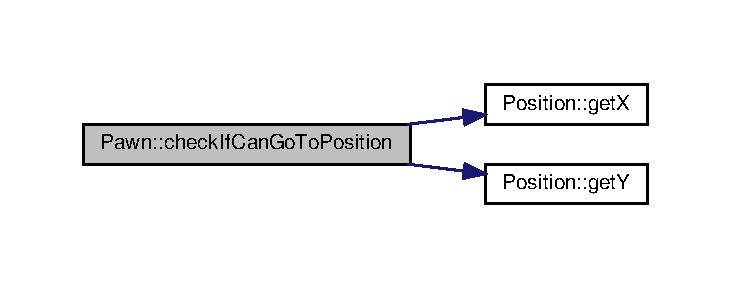
\includegraphics[width=350pt]{classPawn_a30abb1fc67dffcd5f9ae104baf3e27ac_cgraph}
\end{center}
\end{figure}


The documentation for this class was generated from the following files\+:\begin{DoxyCompactItemize}
\item 
include/\hyperlink{Pawn_8h}{Pawn.\+h}\item 
src/\hyperlink{Pawn_8cpp}{Pawn.\+cpp}\end{DoxyCompactItemize}

\hypertarget{classPlayer}{}\section{Player Class Reference}
\label{classPlayer}\index{Player@{Player}}


Class responsible for handling player info.  




{\ttfamily \#include $<$Player.\+h$>$}

\subsection*{Public Member Functions}
\begin{DoxyCompactItemize}
\item 
\hyperlink{classPlayer_a0e6411e555691354341782b0d6b1bc09}{Player} (std\+::string name, \hyperlink{Enums_8h_ab87bacfdad76e61b9412d7124be44c1c}{Color} color)
\begin{DoxyCompactList}\small\item\em Constructor. \end{DoxyCompactList}\item 
std\+::string \hyperlink{classPlayer_af1aa472885d589516f483e26e786600e}{get\+Name} ()
\begin{DoxyCompactList}\small\item\em Returns players name. \end{DoxyCompactList}\item 
\hyperlink{Enums_8h_ab87bacfdad76e61b9412d7124be44c1c}{Color} \hyperlink{classPlayer_abe2b0f82bdfeda3d872c772da40d5140}{get\+Color} ()
\begin{DoxyCompactList}\small\item\em Returns players color. \end{DoxyCompactList}\end{DoxyCompactItemize}


\subsection{Detailed Description}
Class responsible for handling player info. 

\subsection{Constructor \& Destructor Documentation}
\mbox{\Hypertarget{classPlayer_a0e6411e555691354341782b0d6b1bc09}\label{classPlayer_a0e6411e555691354341782b0d6b1bc09}} 
\index{Player@{Player}!Player@{Player}}
\index{Player@{Player}!Player@{Player}}
\subsubsection{\texorpdfstring{Player()}{Player()}}
{\footnotesize\ttfamily Player\+::\+Player (\begin{DoxyParamCaption}\item[{std\+::string}]{name,  }\item[{\hyperlink{Enums_8h_ab87bacfdad76e61b9412d7124be44c1c}{Color}}]{color }\end{DoxyParamCaption})}



Constructor. 


\begin{DoxyParams}{Parameters}
{\em name} & \\
\hline
{\em color} & \\
\hline
\end{DoxyParams}


\subsection{Member Function Documentation}
\mbox{\Hypertarget{classPlayer_abe2b0f82bdfeda3d872c772da40d5140}\label{classPlayer_abe2b0f82bdfeda3d872c772da40d5140}} 
\index{Player@{Player}!get\+Color@{get\+Color}}
\index{get\+Color@{get\+Color}!Player@{Player}}
\subsubsection{\texorpdfstring{get\+Color()}{getColor()}}
{\footnotesize\ttfamily \hyperlink{Enums_8h_ab87bacfdad76e61b9412d7124be44c1c}{Color} Player\+::get\+Color (\begin{DoxyParamCaption}{ }\end{DoxyParamCaption})}



Returns players color. 

\begin{DoxyReturn}{Returns}

\end{DoxyReturn}
\mbox{\Hypertarget{classPlayer_af1aa472885d589516f483e26e786600e}\label{classPlayer_af1aa472885d589516f483e26e786600e}} 
\index{Player@{Player}!get\+Name@{get\+Name}}
\index{get\+Name@{get\+Name}!Player@{Player}}
\subsubsection{\texorpdfstring{get\+Name()}{getName()}}
{\footnotesize\ttfamily std\+::string Player\+::get\+Name (\begin{DoxyParamCaption}{ }\end{DoxyParamCaption})}



Returns players name. 

\begin{DoxyReturn}{Returns}

\end{DoxyReturn}


The documentation for this class was generated from the following files\+:\begin{DoxyCompactItemize}
\item 
include/\hyperlink{Player_8h}{Player.\+h}\item 
src/\hyperlink{Player_8cpp}{Player.\+cpp}\end{DoxyCompactItemize}

\hypertarget{classPosition}{}\section{Position Class Reference}
\label{classPosition}\index{Position@{Position}}


Class responsible for handling position info.  




{\ttfamily \#include $<$Position.\+h$>$}

\subsection*{Public Member Functions}
\begin{DoxyCompactItemize}
\item 
\hyperlink{classPosition_a6e36cf0fee251e74cfedb86f4e99558d}{Position} (int x, int y)
\begin{DoxyCompactList}\small\item\em Constructor. \end{DoxyCompactList}\item 
int \hyperlink{classPosition_a4e65d4b865c08791302956e2912a2300}{getX} ()
\begin{DoxyCompactList}\small\item\em Returns x of position. \end{DoxyCompactList}\item 
int \hyperlink{classPosition_ab386f9a955ea2e291774f8d403614260}{getY} ()
\begin{DoxyCompactList}\small\item\em Returns y of position. \end{DoxyCompactList}\item 
\mbox{\Hypertarget{classPosition_ad46bb77324e2d9538e15f1a25320f1ff}\label{classPosition_ad46bb77324e2d9538e15f1a25320f1ff}} 
void {\bfseries setX} (int x)
\item 
\mbox{\Hypertarget{classPosition_a473274f1a3e4888f9c5e3eba0889a1ab}\label{classPosition_a473274f1a3e4888f9c5e3eba0889a1ab}} 
void {\bfseries setY} (int y)
\end{DoxyCompactItemize}


\subsection{Detailed Description}
Class responsible for handling position info. 

\subsection{Constructor \& Destructor Documentation}
\mbox{\Hypertarget{classPosition_a6e36cf0fee251e74cfedb86f4e99558d}\label{classPosition_a6e36cf0fee251e74cfedb86f4e99558d}} 
\index{Position@{Position}!Position@{Position}}
\index{Position@{Position}!Position@{Position}}
\subsubsection{\texorpdfstring{Position()}{Position()}}
{\footnotesize\ttfamily Position\+::\+Position (\begin{DoxyParamCaption}\item[{int}]{x,  }\item[{int}]{y }\end{DoxyParamCaption})\hspace{0.3cm}{\ttfamily [inline]}}



Constructor. 


\begin{DoxyParams}{Parameters}
{\em x} & \\
\hline
{\em y} & \\
\hline
\end{DoxyParams}
Here is the call graph for this function\+:\nopagebreak
\begin{figure}[H]
\begin{center}
\leavevmode
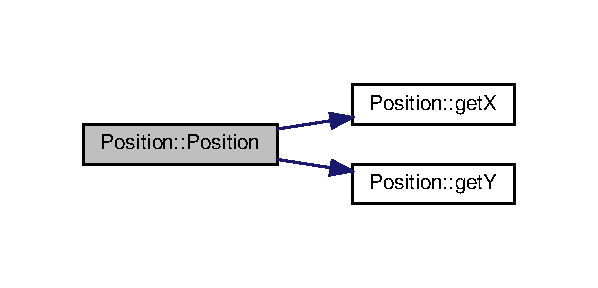
\includegraphics[width=287pt]{classPosition_a6e36cf0fee251e74cfedb86f4e99558d_cgraph}
\end{center}
\end{figure}


\subsection{Member Function Documentation}
\mbox{\Hypertarget{classPosition_a4e65d4b865c08791302956e2912a2300}\label{classPosition_a4e65d4b865c08791302956e2912a2300}} 
\index{Position@{Position}!getX@{getX}}
\index{getX@{getX}!Position@{Position}}
\subsubsection{\texorpdfstring{get\+X()}{getX()}}
{\footnotesize\ttfamily int Position\+::getX (\begin{DoxyParamCaption}{ }\end{DoxyParamCaption})}



Returns x of position. 

\begin{DoxyReturn}{Returns}

\end{DoxyReturn}
\mbox{\Hypertarget{classPosition_ab386f9a955ea2e291774f8d403614260}\label{classPosition_ab386f9a955ea2e291774f8d403614260}} 
\index{Position@{Position}!getY@{getY}}
\index{getY@{getY}!Position@{Position}}
\subsubsection{\texorpdfstring{get\+Y()}{getY()}}
{\footnotesize\ttfamily int Position\+::getY (\begin{DoxyParamCaption}{ }\end{DoxyParamCaption})}



Returns y of position. 

\begin{DoxyReturn}{Returns}

\end{DoxyReturn}


The documentation for this class was generated from the following files\+:\begin{DoxyCompactItemize}
\item 
include/\hyperlink{Position_8h}{Position.\+h}\item 
src/\hyperlink{Position_8cpp}{Position.\+cpp}\end{DoxyCompactItemize}

\hypertarget{classQueen}{}\section{Queen Class Reference}
\label{classQueen}\index{Queen@{Queen}}


Class responsible for queen chess piece actions.  




{\ttfamily \#include $<$Queen.\+h$>$}



Inheritance diagram for Queen\+:\nopagebreak
\begin{figure}[H]
\begin{center}
\leavevmode
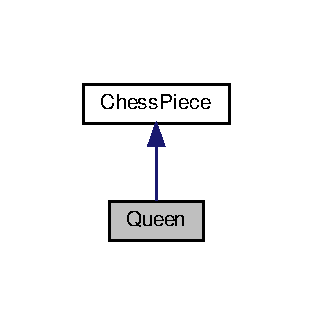
\includegraphics[width=150pt]{classQueen__inherit__graph}
\end{center}
\end{figure}


Collaboration diagram for Queen\+:\nopagebreak
\begin{figure}[H]
\begin{center}
\leavevmode
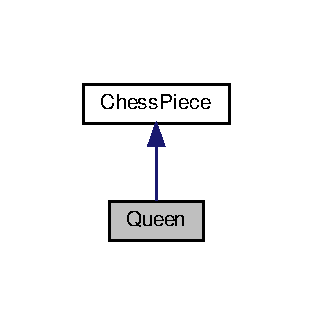
\includegraphics[width=150pt]{classQueen__coll__graph}
\end{center}
\end{figure}
\subsection*{Public Member Functions}
\begin{DoxyCompactItemize}
\item 
\hyperlink{classQueen_ae4b3b4f515f2024e1f554369332fa834}{Queen} (\hyperlink{Enums_8h_ab87bacfdad76e61b9412d7124be44c1c}{Color} \hyperlink{classChessPiece_a8c8fc170e7c719ac2b71a93a56a38f01}{color})
\begin{DoxyCompactList}\small\item\em Constructor. \end{DoxyCompactList}\item 
bool \hyperlink{classQueen_a504eb0f657c4ae6acbf54ef8ab4c5cf9}{check\+If\+Can\+Go\+To\+Position} (\hyperlink{classPosition}{Position} from\+Position, \hyperlink{classPosition}{Position} to\+Position, \hyperlink{classBoard}{Board} $\ast$board)
\begin{DoxyCompactList}\small\item\em Checks if queen can go form from\+Position to to\+Position. \end{DoxyCompactList}\end{DoxyCompactItemize}
\subsection*{Additional Inherited Members}


\subsection{Detailed Description}
Class responsible for queen chess piece actions. 

\subsection{Constructor \& Destructor Documentation}
\mbox{\Hypertarget{classQueen_ae4b3b4f515f2024e1f554369332fa834}\label{classQueen_ae4b3b4f515f2024e1f554369332fa834}} 
\index{Queen@{Queen}!Queen@{Queen}}
\index{Queen@{Queen}!Queen@{Queen}}
\subsubsection{\texorpdfstring{Queen()}{Queen()}}
{\footnotesize\ttfamily Queen\+::\+Queen (\begin{DoxyParamCaption}\item[{\hyperlink{Enums_8h_ab87bacfdad76e61b9412d7124be44c1c}{Color}}]{color }\end{DoxyParamCaption})\hspace{0.3cm}{\ttfamily [inline]}}



Constructor. 


\begin{DoxyParams}{Parameters}
{\em color} & \\
\hline
\end{DoxyParams}
Here is the call graph for this function\+:
\nopagebreak
\begin{figure}[H]
\begin{center}
\leavevmode
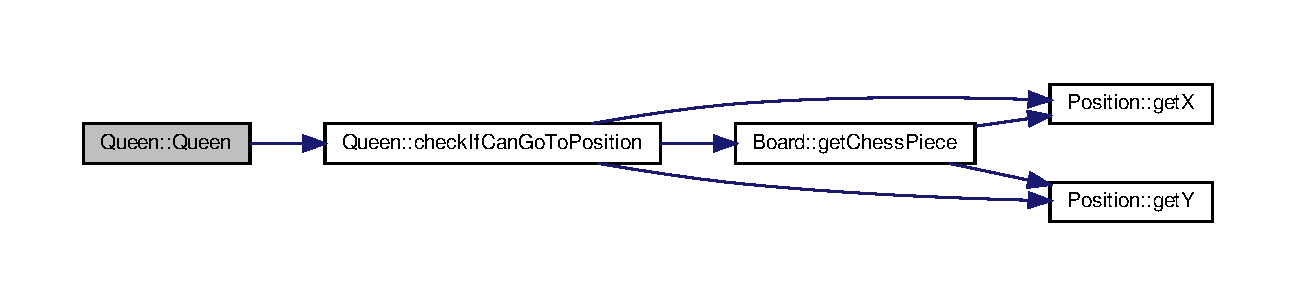
\includegraphics[width=350pt]{classQueen_ae4b3b4f515f2024e1f554369332fa834_cgraph}
\end{center}
\end{figure}


\subsection{Member Function Documentation}
\mbox{\Hypertarget{classQueen_a504eb0f657c4ae6acbf54ef8ab4c5cf9}\label{classQueen_a504eb0f657c4ae6acbf54ef8ab4c5cf9}} 
\index{Queen@{Queen}!check\+If\+Can\+Go\+To\+Position@{check\+If\+Can\+Go\+To\+Position}}
\index{check\+If\+Can\+Go\+To\+Position@{check\+If\+Can\+Go\+To\+Position}!Queen@{Queen}}
\subsubsection{\texorpdfstring{check\+If\+Can\+Go\+To\+Position()}{checkIfCanGoToPosition()}}
{\footnotesize\ttfamily bool Queen\+::check\+If\+Can\+Go\+To\+Position (\begin{DoxyParamCaption}\item[{\hyperlink{classPosition}{Position}}]{from\+Position,  }\item[{\hyperlink{classPosition}{Position}}]{to\+Position,  }\item[{\hyperlink{classBoard}{Board} $\ast$}]{board }\end{DoxyParamCaption})\hspace{0.3cm}{\ttfamily [virtual]}}



Checks if queen can go form from\+Position to to\+Position. 


\begin{DoxyParams}{Parameters}
{\em from\+Position} & \\
\hline
{\em to\+Position} & \\
\hline
{\em board} & \\
\hline
\end{DoxyParams}
\begin{DoxyReturn}{Returns}

\end{DoxyReturn}


Implements \hyperlink{classChessPiece_a90119a7c3c74ed9f967c398b8a7d7a98}{Chess\+Piece}.

Here is the call graph for this function\+:
\nopagebreak
\begin{figure}[H]
\begin{center}
\leavevmode
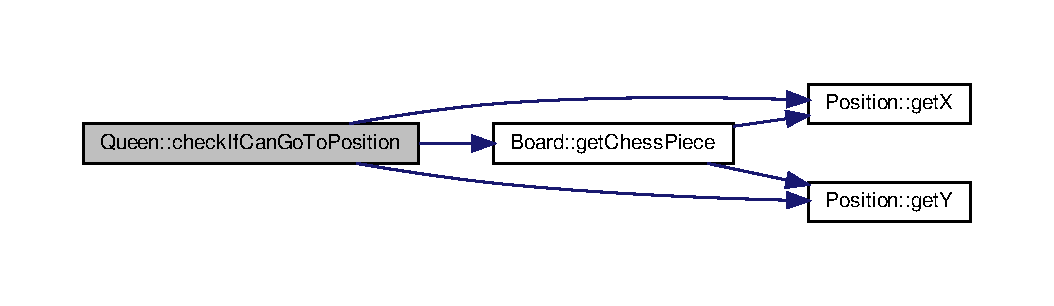
\includegraphics[width=350pt]{classQueen_a504eb0f657c4ae6acbf54ef8ab4c5cf9_cgraph}
\end{center}
\end{figure}


The documentation for this class was generated from the following files\+:\begin{DoxyCompactItemize}
\item 
include/\hyperlink{Queen_8h}{Queen.\+h}\item 
src/\hyperlink{Queen_8cpp}{Queen.\+cpp}\end{DoxyCompactItemize}

\hypertarget{classRook}{}\section{Rook Class Reference}
\label{classRook}\index{Rook@{Rook}}


Class responsible for rook chess piece actions.  




{\ttfamily \#include $<$Rook.\+h$>$}



Inheritance diagram for Rook\+:\nopagebreak
\begin{figure}[H]
\begin{center}
\leavevmode
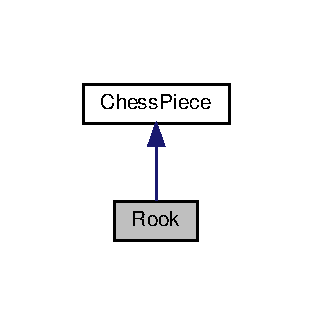
\includegraphics[width=150pt]{classRook__inherit__graph}
\end{center}
\end{figure}


Collaboration diagram for Rook\+:\nopagebreak
\begin{figure}[H]
\begin{center}
\leavevmode
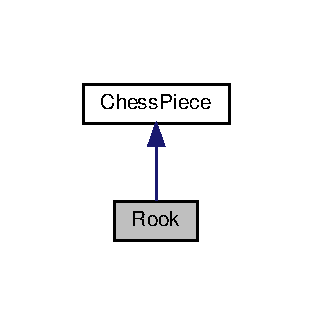
\includegraphics[width=150pt]{classRook__coll__graph}
\end{center}
\end{figure}
\subsection*{Public Member Functions}
\begin{DoxyCompactItemize}
\item 
\hyperlink{classRook_ad737fa250eb3e4d1a312d9bceda6a9cd}{Rook} (\hyperlink{Enums_8h_ab87bacfdad76e61b9412d7124be44c1c}{Color} \hyperlink{classChessPiece_a8c8fc170e7c719ac2b71a93a56a38f01}{color})
\begin{DoxyCompactList}\small\item\em Constructor. \end{DoxyCompactList}\item 
bool \hyperlink{classRook_aad67c9012197bf285cf6a27861fbcb06}{check\+If\+Can\+Go\+To\+Position} (\hyperlink{classPosition}{Position} from\+Position, \hyperlink{classPosition}{Position} to\+Position, \hyperlink{classBoard}{Board} $\ast$board)
\begin{DoxyCompactList}\small\item\em Checks if rook can go form from\+Position to to\+Position. \end{DoxyCompactList}\end{DoxyCompactItemize}
\subsection*{Additional Inherited Members}


\subsection{Detailed Description}
Class responsible for rook chess piece actions. 

\subsection{Constructor \& Destructor Documentation}
\mbox{\Hypertarget{classRook_ad737fa250eb3e4d1a312d9bceda6a9cd}\label{classRook_ad737fa250eb3e4d1a312d9bceda6a9cd}} 
\index{Rook@{Rook}!Rook@{Rook}}
\index{Rook@{Rook}!Rook@{Rook}}
\subsubsection{\texorpdfstring{Rook()}{Rook()}}
{\footnotesize\ttfamily Rook\+::\+Rook (\begin{DoxyParamCaption}\item[{\hyperlink{Enums_8h_ab87bacfdad76e61b9412d7124be44c1c}{Color}}]{color }\end{DoxyParamCaption})\hspace{0.3cm}{\ttfamily [inline]}}



Constructor. 


\begin{DoxyParams}{Parameters}
{\em color} & \\
\hline
\end{DoxyParams}
Here is the call graph for this function\+:
\nopagebreak
\begin{figure}[H]
\begin{center}
\leavevmode
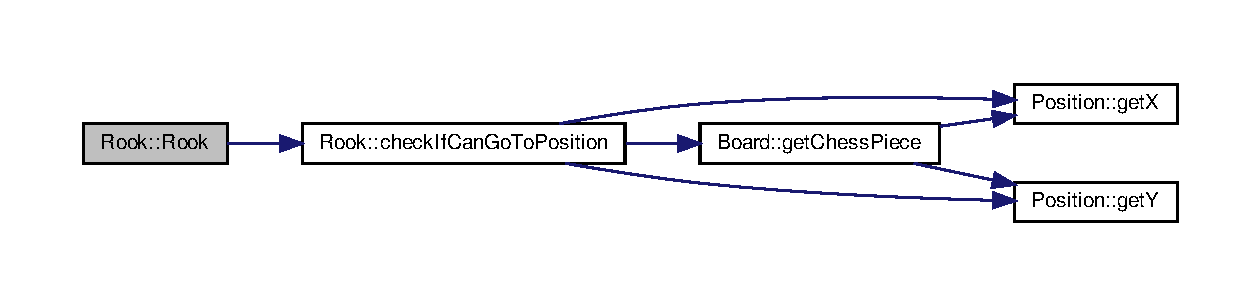
\includegraphics[width=350pt]{classRook_ad737fa250eb3e4d1a312d9bceda6a9cd_cgraph}
\end{center}
\end{figure}


\subsection{Member Function Documentation}
\mbox{\Hypertarget{classRook_aad67c9012197bf285cf6a27861fbcb06}\label{classRook_aad67c9012197bf285cf6a27861fbcb06}} 
\index{Rook@{Rook}!check\+If\+Can\+Go\+To\+Position@{check\+If\+Can\+Go\+To\+Position}}
\index{check\+If\+Can\+Go\+To\+Position@{check\+If\+Can\+Go\+To\+Position}!Rook@{Rook}}
\subsubsection{\texorpdfstring{check\+If\+Can\+Go\+To\+Position()}{checkIfCanGoToPosition()}}
{\footnotesize\ttfamily bool Rook\+::check\+If\+Can\+Go\+To\+Position (\begin{DoxyParamCaption}\item[{\hyperlink{classPosition}{Position}}]{from\+Position,  }\item[{\hyperlink{classPosition}{Position}}]{to\+Position,  }\item[{\hyperlink{classBoard}{Board} $\ast$}]{board }\end{DoxyParamCaption})\hspace{0.3cm}{\ttfamily [virtual]}}



Checks if rook can go form from\+Position to to\+Position. 


\begin{DoxyParams}{Parameters}
{\em from\+Position} & \\
\hline
{\em to\+Position} & \\
\hline
{\em board} & \\
\hline
\end{DoxyParams}
\begin{DoxyReturn}{Returns}

\end{DoxyReturn}


Implements \hyperlink{classChessPiece_a90119a7c3c74ed9f967c398b8a7d7a98}{Chess\+Piece}.

Here is the call graph for this function\+:
\nopagebreak
\begin{figure}[H]
\begin{center}
\leavevmode
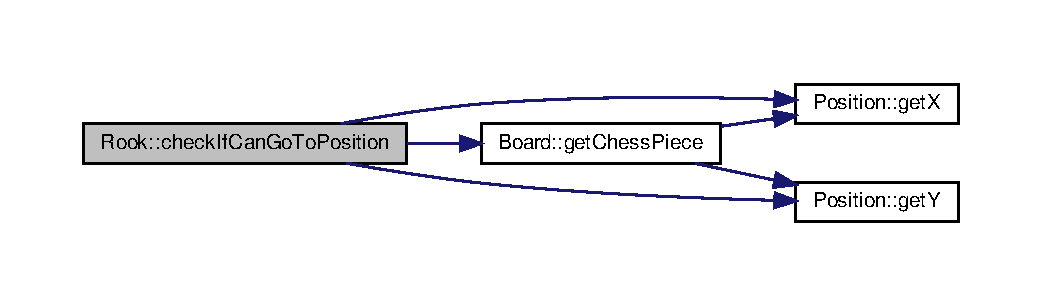
\includegraphics[width=350pt]{classRook_aad67c9012197bf285cf6a27861fbcb06_cgraph}
\end{center}
\end{figure}


The documentation for this class was generated from the following files\+:\begin{DoxyCompactItemize}
\item 
include/\hyperlink{Rook_8h}{Rook.\+h}\item 
src/\hyperlink{Rook_8cpp}{Rook.\+cpp}\end{DoxyCompactItemize}

\chapter{File Documentation}
\hypertarget{Bishop_8h}{}\section{include/\+Bishop.h File Reference}
\label{Bishop_8h}\index{include/\+Bishop.\+h@{include/\+Bishop.\+h}}
{\ttfamily \#include \char`\"{}Chess\+Piece.\+h\char`\"{}}\newline
Include dependency graph for Bishop.\+h\+:\nopagebreak
\begin{figure}[H]
\begin{center}
\leavevmode
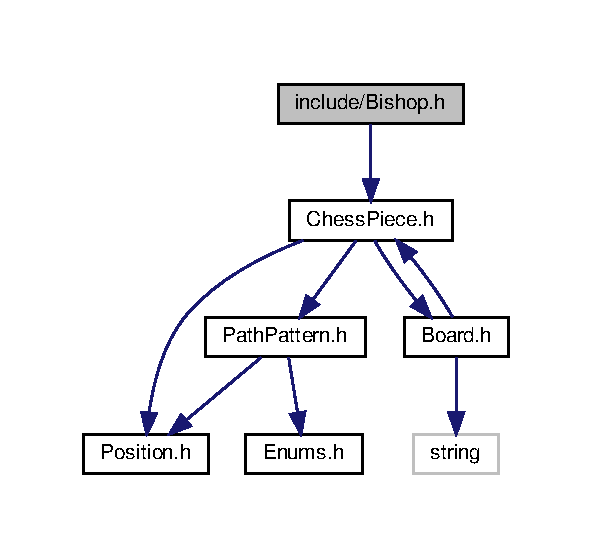
\includegraphics[width=284pt]{Bishop_8h__incl}
\end{center}
\end{figure}
This graph shows which files directly or indirectly include this file\+:\nopagebreak
\begin{figure}[H]
\begin{center}
\leavevmode
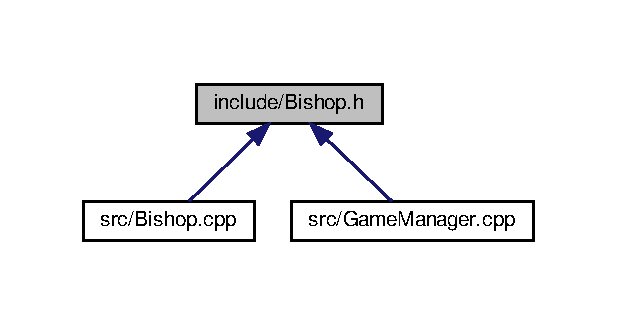
\includegraphics[width=296pt]{Bishop_8h__dep__incl}
\end{center}
\end{figure}
\subsection*{Classes}
\begin{DoxyCompactItemize}
\item 
class \hyperlink{classBishop}{Bishop}
\begin{DoxyCompactList}\small\item\em Class responsible for handling bishop chess piece actions. \end{DoxyCompactList}\end{DoxyCompactItemize}

\hypertarget{Board_8h}{}\section{include/\+Board.h File Reference}
\label{Board_8h}\index{include/\+Board.\+h@{include/\+Board.\+h}}
{\ttfamily \#include $<$string$>$}\newline
{\ttfamily \#include \char`\"{}Chess\+Piece.\+h\char`\"{}}\newline
Include dependency graph for Board.\+h\+:\nopagebreak
\begin{figure}[H]
\begin{center}
\leavevmode
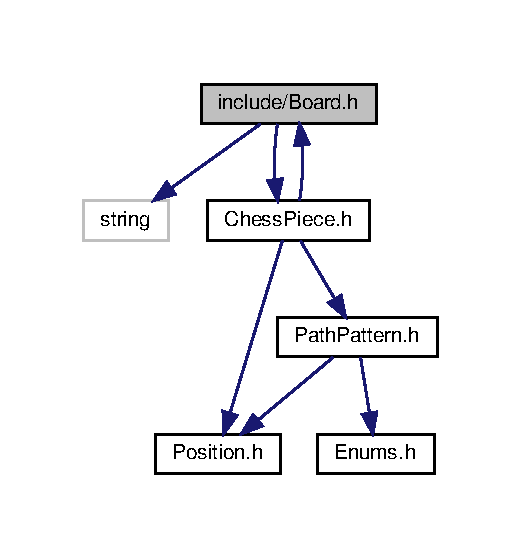
\includegraphics[width=250pt]{Board_8h__incl}
\end{center}
\end{figure}
This graph shows which files directly or indirectly include this file\+:\nopagebreak
\begin{figure}[H]
\begin{center}
\leavevmode
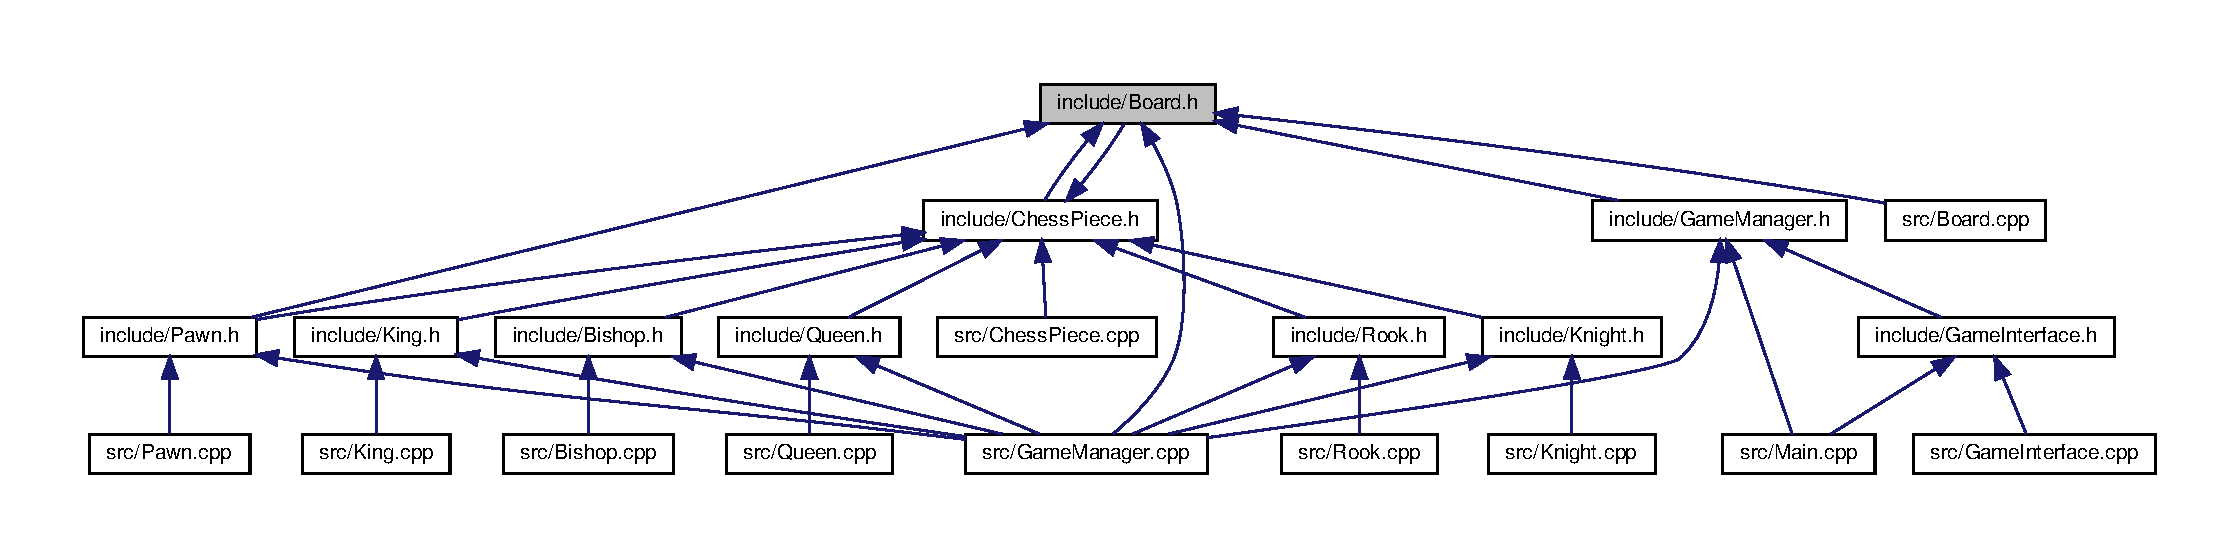
\includegraphics[width=350pt]{Board_8h__dep__incl}
\end{center}
\end{figure}
\subsection*{Classes}
\begin{DoxyCompactItemize}
\item 
class \hyperlink{classBoard}{Board}
\begin{DoxyCompactList}\small\item\em Class responsible for handling board and board actions. \end{DoxyCompactList}\end{DoxyCompactItemize}
\subsection*{Macros}
\begin{DoxyCompactItemize}
\item 
\mbox{\Hypertarget{Board_8h_a1db39eb31d1315ce982608fe25587b6d}\label{Board_8h_a1db39eb31d1315ce982608fe25587b6d}} 
\#define {\bfseries B\+O\+A\+R\+D\+\_\+\+S\+I\+ZE}~8
\end{DoxyCompactItemize}

\hypertarget{ChessPiece_8h}{}\section{include/\+Chess\+Piece.h File Reference}
\label{ChessPiece_8h}\index{include/\+Chess\+Piece.\+h@{include/\+Chess\+Piece.\+h}}
{\ttfamily \#include \char`\"{}Position.\+h\char`\"{}}\newline
{\ttfamily \#include \char`\"{}Path\+Pattern.\+h\char`\"{}}\newline
{\ttfamily \#include \char`\"{}Board.\+h\char`\"{}}\newline
Include dependency graph for Chess\+Piece.\+h\+:\nopagebreak
\begin{figure}[H]
\begin{center}
\leavevmode
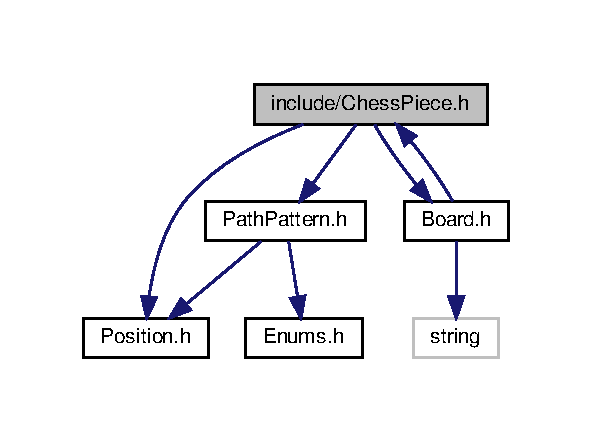
\includegraphics[width=284pt]{ChessPiece_8h__incl}
\end{center}
\end{figure}
This graph shows which files directly or indirectly include this file\+:\nopagebreak
\begin{figure}[H]
\begin{center}
\leavevmode
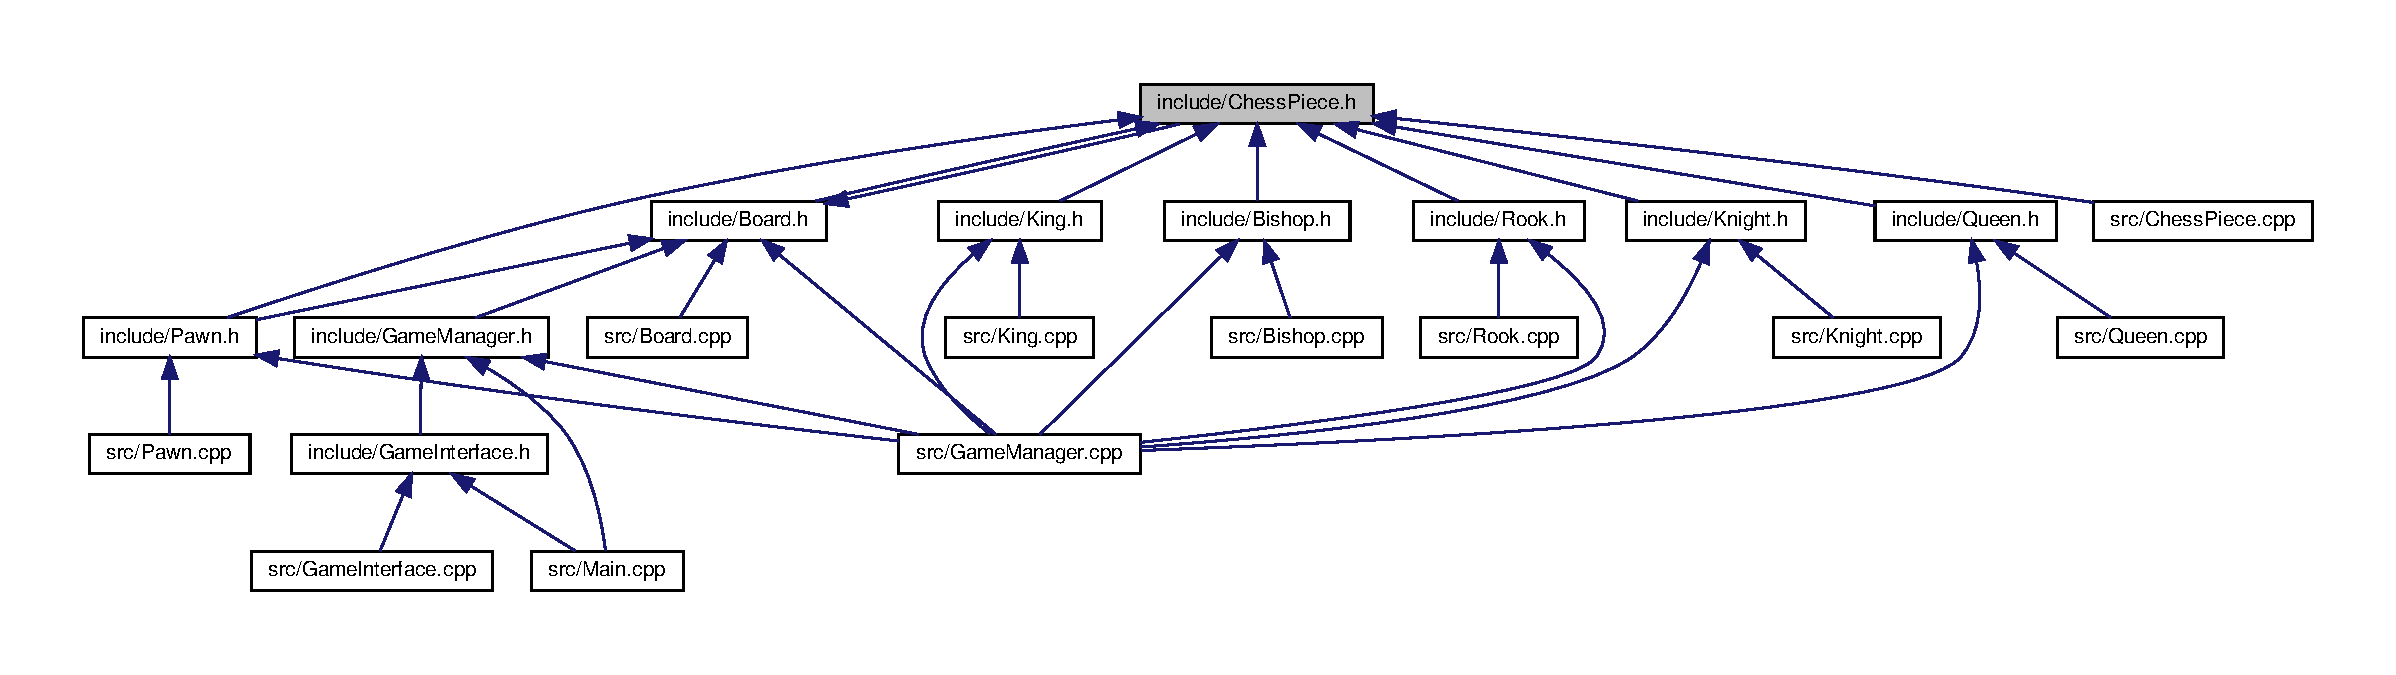
\includegraphics[width=350pt]{ChessPiece_8h__dep__incl}
\end{center}
\end{figure}
\subsection*{Classes}
\begin{DoxyCompactItemize}
\item 
class \hyperlink{classChessPiece}{Chess\+Piece}
\begin{DoxyCompactList}\small\item\em Class responsible for basic chess piece actions. \end{DoxyCompactList}\end{DoxyCompactItemize}

\hypertarget{Enums_8h}{}\section{include/\+Enums.h File Reference}
\label{Enums_8h}\index{include/\+Enums.\+h@{include/\+Enums.\+h}}


Handling enums of the project.  


This graph shows which files directly or indirectly include this file\+:\nopagebreak
\begin{figure}[H]
\begin{center}
\leavevmode
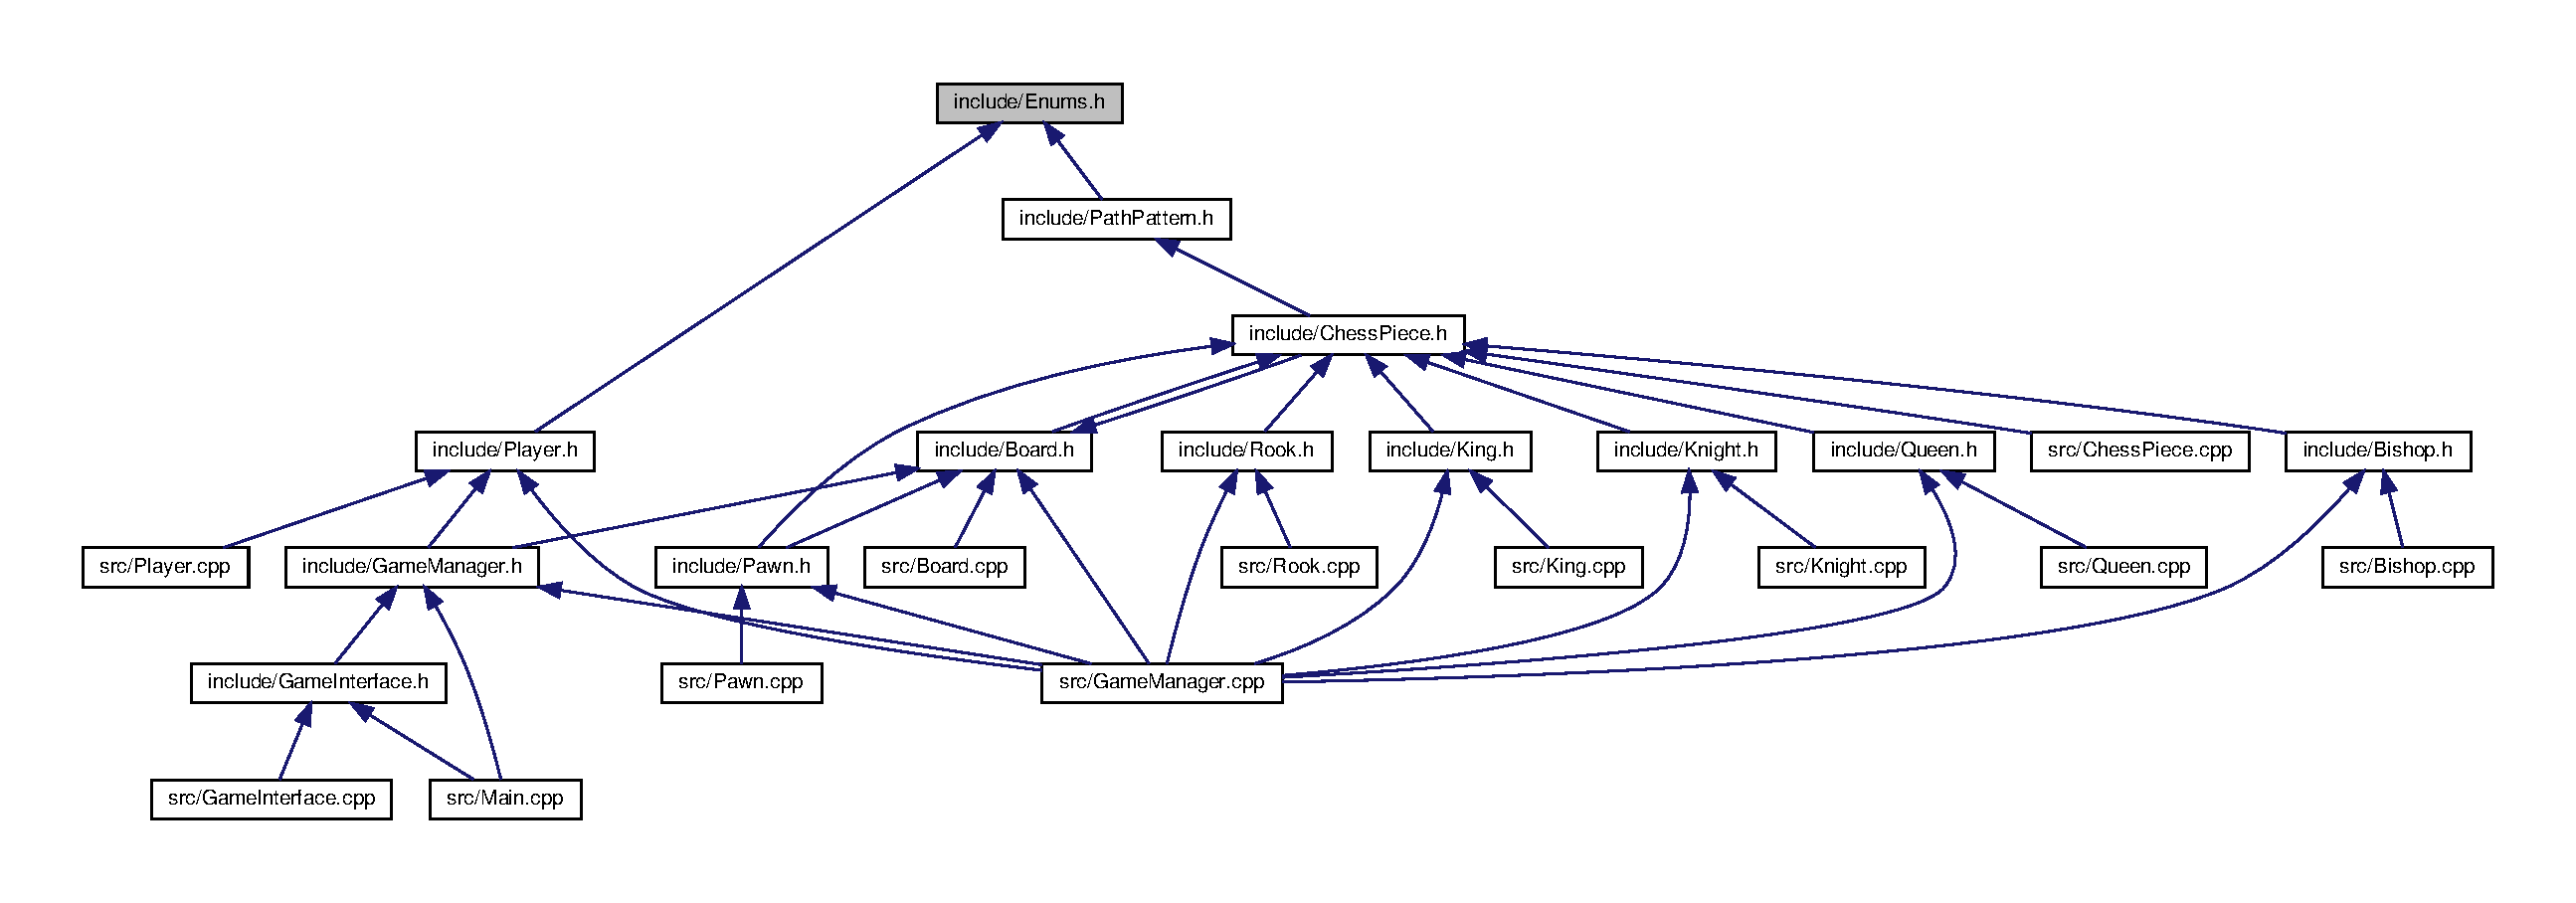
\includegraphics[width=350pt]{Enums_8h__dep__incl}
\end{center}
\end{figure}
\subsection*{Typedefs}
\begin{DoxyCompactItemize}
\item 
\mbox{\Hypertarget{Enums_8h_ad196bf510b28a9ba4c872e96dfd16f92}\label{Enums_8h_ad196bf510b28a9ba4c872e96dfd16f92}} 
typedef enum \hyperlink{Enums_8h_a224b9163917ac32fc95a60d8c1eec3aa}{Direction} {\bfseries Direction}
\item 
\mbox{\Hypertarget{Enums_8h_a8b6b3870db501097758d25d7f3a2c95f}\label{Enums_8h_a8b6b3870db501097758d25d7f3a2c95f}} 
typedef enum \hyperlink{Enums_8h_ab87bacfdad76e61b9412d7124be44c1c}{Color} {\bfseries Color}
\end{DoxyCompactItemize}
\subsection*{Enumerations}
\begin{DoxyCompactItemize}
\item 
\mbox{\Hypertarget{Enums_8h_a224b9163917ac32fc95a60d8c1eec3aa}\label{Enums_8h_a224b9163917ac32fc95a60d8c1eec3aa}} 
enum \hyperlink{Enums_8h_a224b9163917ac32fc95a60d8c1eec3aa}{Direction} \{ \newline
{\bfseries UP} = 1, 
{\bfseries U\+P\+\_\+\+R\+I\+G\+HT}, 
{\bfseries R\+I\+G\+HT}, 
{\bfseries R\+I\+G\+H\+T\+\_\+\+D\+O\+WN}, 
\newline
{\bfseries D\+O\+WN} =-\/1, 
{\bfseries D\+O\+W\+N\+\_\+\+L\+E\+FT}, 
{\bfseries L\+E\+FT}, 
{\bfseries L\+E\+F\+T\+\_\+\+UP}
 \}\begin{DoxyCompactList}\small\item\em Enum dedicated to directions. \end{DoxyCompactList}
\item 
\mbox{\Hypertarget{Enums_8h_ab87bacfdad76e61b9412d7124be44c1c}\label{Enums_8h_ab87bacfdad76e61b9412d7124be44c1c}} 
enum \hyperlink{Enums_8h_ab87bacfdad76e61b9412d7124be44c1c}{Color} \{ {\bfseries W\+H\+I\+TE}, 
{\bfseries B\+L\+A\+CK}
 \}\begin{DoxyCompactList}\small\item\em Enum dedicated to colors. \end{DoxyCompactList}
\end{DoxyCompactItemize}


\subsection{Detailed Description}
Handling enums of the project. 


\hypertarget{GameInterface_8h}{}\section{include/\+Game\+Interface.h File Reference}
\label{GameInterface_8h}\index{include/\+Game\+Interface.\+h@{include/\+Game\+Interface.\+h}}
{\ttfamily \#include \char`\"{}Game\+Manager.\+h\char`\"{}}\newline
Include dependency graph for Game\+Interface.\+h\+:\nopagebreak
\begin{figure}[H]
\begin{center}
\leavevmode
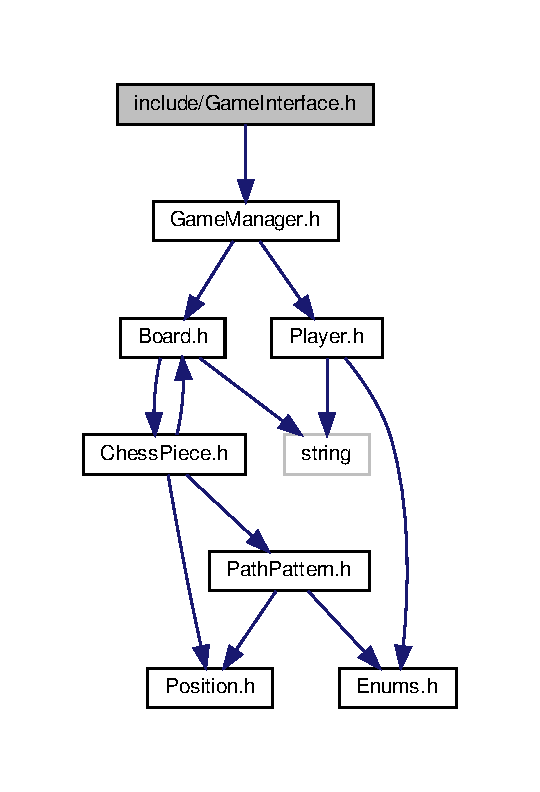
\includegraphics[width=259pt]{GameInterface_8h__incl}
\end{center}
\end{figure}
This graph shows which files directly or indirectly include this file\+:\nopagebreak
\begin{figure}[H]
\begin{center}
\leavevmode
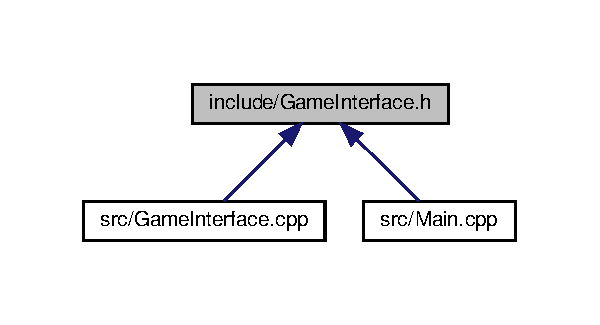
\includegraphics[width=288pt]{GameInterface_8h__dep__incl}
\end{center}
\end{figure}
\subsection*{Classes}
\begin{DoxyCompactItemize}
\item 
class \hyperlink{classGameInterface}{Game\+Interface}
\begin{DoxyCompactList}\small\item\em Class responsible for user interface. \end{DoxyCompactList}\end{DoxyCompactItemize}

\hypertarget{GameManager_8h}{}\section{include/\+Game\+Manager.h File Reference}
\label{GameManager_8h}\index{include/\+Game\+Manager.\+h@{include/\+Game\+Manager.\+h}}
{\ttfamily \#include \char`\"{}Board.\+h\char`\"{}}\newline
{\ttfamily \#include \char`\"{}Player.\+h\char`\"{}}\newline
Include dependency graph for Game\+Manager.\+h\+:\nopagebreak
\begin{figure}[H]
\begin{center}
\leavevmode
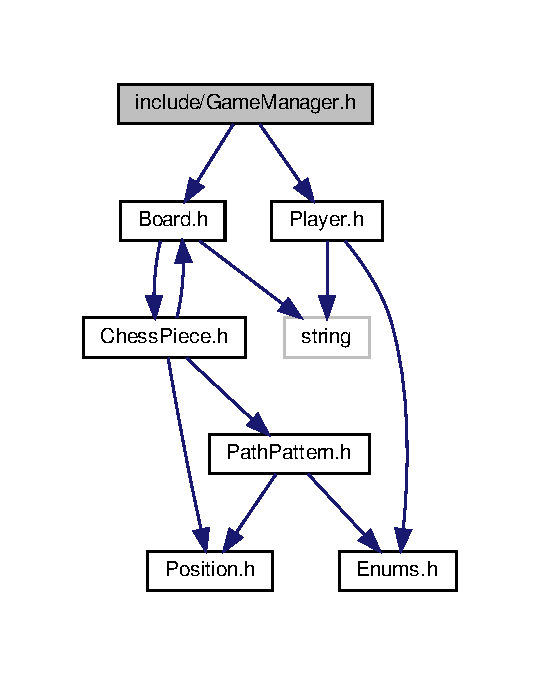
\includegraphics[width=259pt]{GameManager_8h__incl}
\end{center}
\end{figure}
This graph shows which files directly or indirectly include this file\+:\nopagebreak
\begin{figure}[H]
\begin{center}
\leavevmode
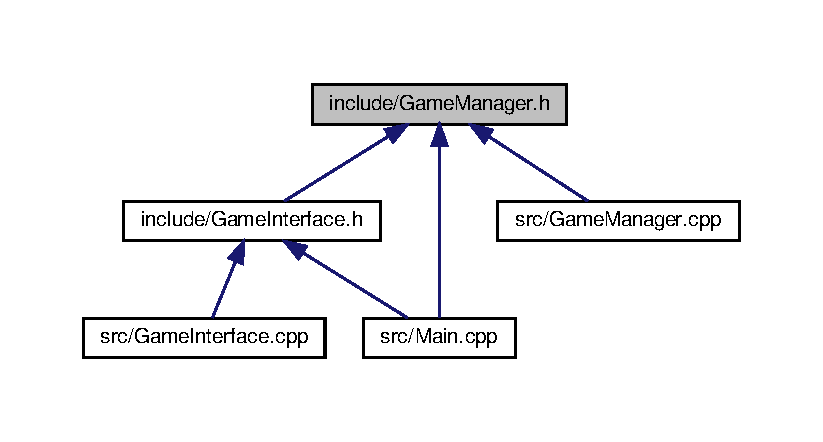
\includegraphics[width=350pt]{GameManager_8h__dep__incl}
\end{center}
\end{figure}
\subsection*{Classes}
\begin{DoxyCompactItemize}
\item 
class \hyperlink{classGameManager}{Game\+Manager}
\begin{DoxyCompactList}\small\item\em Class responsible for managing game logic. \end{DoxyCompactList}\end{DoxyCompactItemize}

\hypertarget{King_8h}{}\section{include/\+King.h File Reference}
\label{King_8h}\index{include/\+King.\+h@{include/\+King.\+h}}
{\ttfamily \#include \char`\"{}Chess\+Piece.\+h\char`\"{}}\newline
Include dependency graph for King.\+h\+:\nopagebreak
\begin{figure}[H]
\begin{center}
\leavevmode
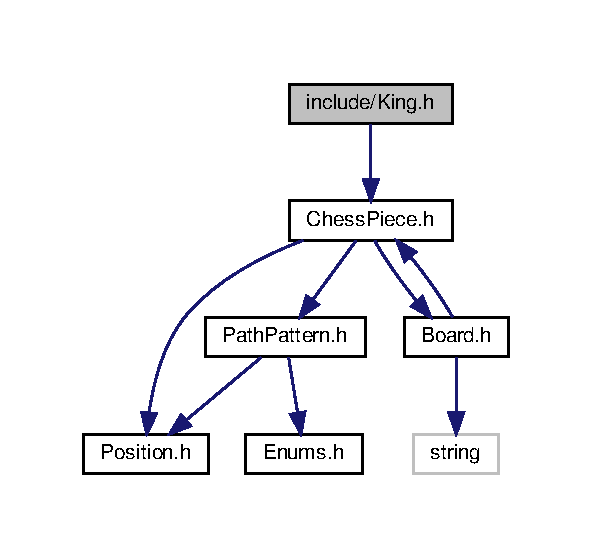
\includegraphics[width=284pt]{King_8h__incl}
\end{center}
\end{figure}
This graph shows which files directly or indirectly include this file\+:\nopagebreak
\begin{figure}[H]
\begin{center}
\leavevmode
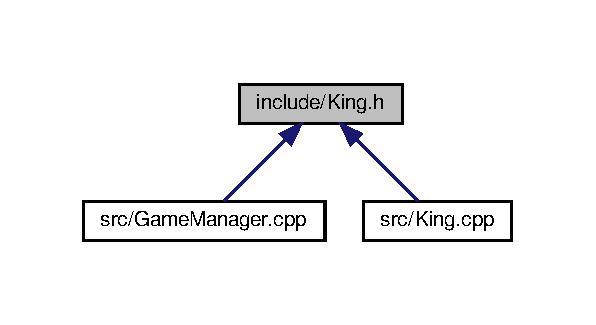
\includegraphics[width=286pt]{King_8h__dep__incl}
\end{center}
\end{figure}
\subsection*{Classes}
\begin{DoxyCompactItemize}
\item 
class \hyperlink{classKing}{King}
\begin{DoxyCompactList}\small\item\em Class responsible for king chess piece actions. \end{DoxyCompactList}\end{DoxyCompactItemize}

\hypertarget{Knight_8h}{}\section{include/\+Knight.h File Reference}
\label{Knight_8h}\index{include/\+Knight.\+h@{include/\+Knight.\+h}}
{\ttfamily \#include \char`\"{}Chess\+Piece.\+h\char`\"{}}\newline
Include dependency graph for Knight.\+h\+:\nopagebreak
\begin{figure}[H]
\begin{center}
\leavevmode
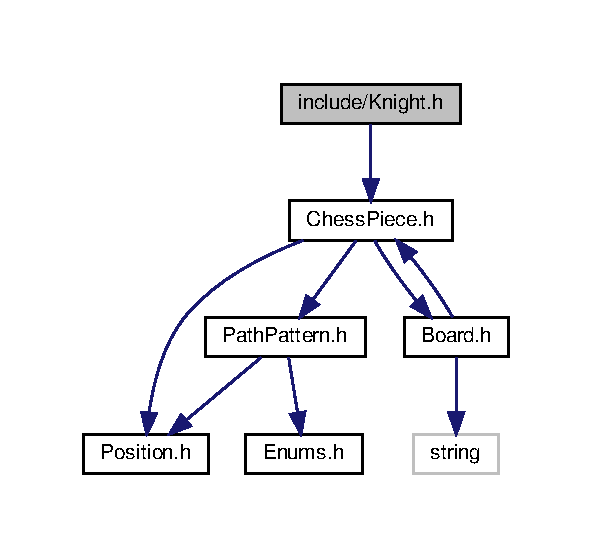
\includegraphics[width=284pt]{Knight_8h__incl}
\end{center}
\end{figure}
This graph shows which files directly or indirectly include this file\+:\nopagebreak
\begin{figure}[H]
\begin{center}
\leavevmode
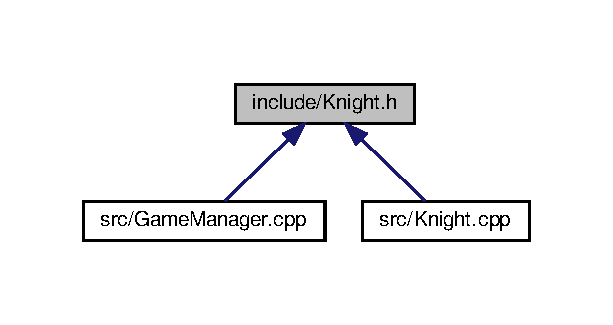
\includegraphics[width=294pt]{Knight_8h__dep__incl}
\end{center}
\end{figure}
\subsection*{Classes}
\begin{DoxyCompactItemize}
\item 
class \hyperlink{classKnight}{Knight}
\begin{DoxyCompactList}\small\item\em Class responsible for knight chess piece actions. \end{DoxyCompactList}\end{DoxyCompactItemize}

\hypertarget{Pawn_8h}{}\section{include/\+Pawn.h File Reference}
\label{Pawn_8h}\index{include/\+Pawn.\+h@{include/\+Pawn.\+h}}
{\ttfamily \#include \char`\"{}Chess\+Piece.\+h\char`\"{}}\newline
{\ttfamily \#include \char`\"{}Board.\+h\char`\"{}}\newline
Include dependency graph for Pawn.\+h\+:\nopagebreak
\begin{figure}[H]
\begin{center}
\leavevmode
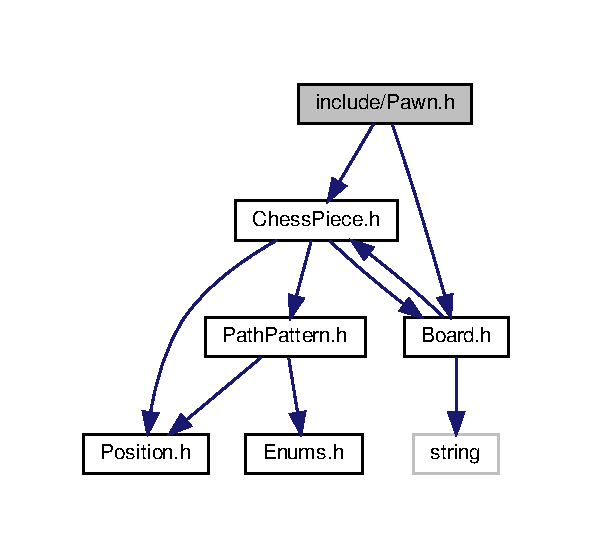
\includegraphics[width=284pt]{Pawn_8h__incl}
\end{center}
\end{figure}
This graph shows which files directly or indirectly include this file\+:\nopagebreak
\begin{figure}[H]
\begin{center}
\leavevmode
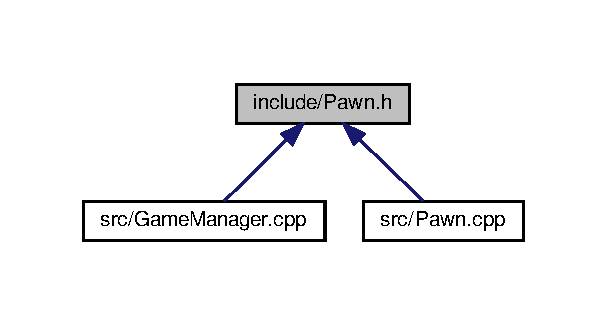
\includegraphics[width=292pt]{Pawn_8h__dep__incl}
\end{center}
\end{figure}
\subsection*{Classes}
\begin{DoxyCompactItemize}
\item 
class \hyperlink{classPawn}{Pawn}
\begin{DoxyCompactList}\small\item\em Class responsible for pawn chess piece actions. \end{DoxyCompactList}\end{DoxyCompactItemize}

\hypertarget{Player_8h}{}\section{include/\+Player.h File Reference}
\label{Player_8h}\index{include/\+Player.\+h@{include/\+Player.\+h}}
{\ttfamily \#include $<$string$>$}\newline
{\ttfamily \#include \char`\"{}Enums.\+h\char`\"{}}\newline
Include dependency graph for Player.\+h\+:\nopagebreak
\begin{figure}[H]
\begin{center}
\leavevmode
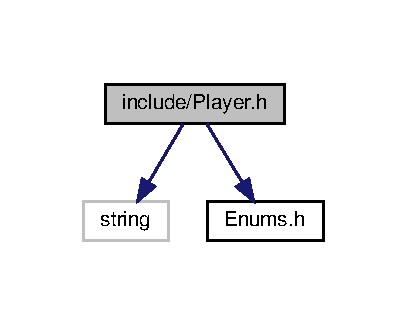
\includegraphics[width=196pt]{Player_8h__incl}
\end{center}
\end{figure}
This graph shows which files directly or indirectly include this file\+:\nopagebreak
\begin{figure}[H]
\begin{center}
\leavevmode
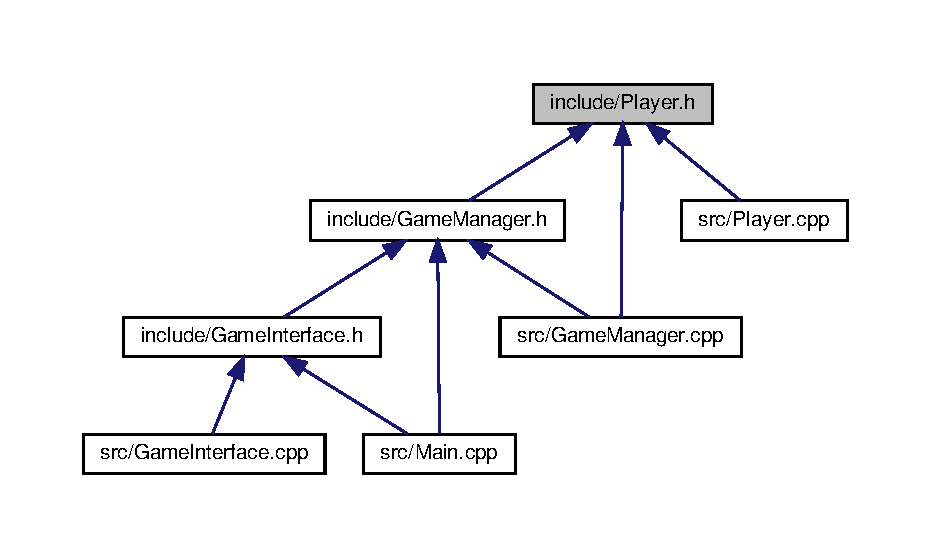
\includegraphics[width=350pt]{Player_8h__dep__incl}
\end{center}
\end{figure}
\subsection*{Classes}
\begin{DoxyCompactItemize}
\item 
class \hyperlink{classPlayer}{Player}
\begin{DoxyCompactList}\small\item\em Class responsible for handling player info. \end{DoxyCompactList}\end{DoxyCompactItemize}

\hypertarget{Position_8h}{}\section{include/\+Position.h File Reference}
\label{Position_8h}\index{include/\+Position.\+h@{include/\+Position.\+h}}
This graph shows which files directly or indirectly include this file\+:\nopagebreak
\begin{figure}[H]
\begin{center}
\leavevmode
\includegraphics[width=350pt]{Position_8h__dep__incl}
\end{center}
\end{figure}
\subsection*{Classes}
\begin{DoxyCompactItemize}
\item 
class \hyperlink{classPosition}{Position}
\begin{DoxyCompactList}\small\item\em Class responsible for handling position info. \end{DoxyCompactList}\end{DoxyCompactItemize}

\hypertarget{Queen_8h}{}\section{include/\+Queen.h File Reference}
\label{Queen_8h}\index{include/\+Queen.\+h@{include/\+Queen.\+h}}
{\ttfamily \#include \char`\"{}Chess\+Piece.\+h\char`\"{}}\newline
Include dependency graph for Queen.\+h\+:\nopagebreak
\begin{figure}[H]
\begin{center}
\leavevmode
\includegraphics[width=284pt]{Queen_8h__incl}
\end{center}
\end{figure}
This graph shows which files directly or indirectly include this file\+:\nopagebreak
\begin{figure}[H]
\begin{center}
\leavevmode
\includegraphics[width=294pt]{Queen_8h__dep__incl}
\end{center}
\end{figure}
\subsection*{Classes}
\begin{DoxyCompactItemize}
\item 
class \hyperlink{classQueen}{Queen}
\begin{DoxyCompactList}\small\item\em Class responsible for queen chess piece actions. \end{DoxyCompactList}\end{DoxyCompactItemize}

\hypertarget{Rook_8h}{}\section{include/\+Rook.h File Reference}
\label{Rook_8h}\index{include/\+Rook.\+h@{include/\+Rook.\+h}}
{\ttfamily \#include \char`\"{}Chess\+Piece.\+h\char`\"{}}\newline
Include dependency graph for Rook.\+h\+:\nopagebreak
\begin{figure}[H]
\begin{center}
\leavevmode
\includegraphics[width=284pt]{Rook_8h__incl}
\end{center}
\end{figure}
This graph shows which files directly or indirectly include this file\+:\nopagebreak
\begin{figure}[H]
\begin{center}
\leavevmode
\includegraphics[width=290pt]{Rook_8h__dep__incl}
\end{center}
\end{figure}
\subsection*{Classes}
\begin{DoxyCompactItemize}
\item 
class \hyperlink{classRook}{Rook}
\begin{DoxyCompactList}\small\item\em Class responsible for rook chess piece actions. \end{DoxyCompactList}\end{DoxyCompactItemize}

\hypertarget{Bishop_8cpp}{}\section{src/\+Bishop.cpp File Reference}
\label{Bishop_8cpp}\index{src/\+Bishop.\+cpp@{src/\+Bishop.\+cpp}}
{\ttfamily \#include $<$cstdlib$>$}\newline
{\ttfamily \#include \char`\"{}../include/\+Bishop.\+h\char`\"{}}\newline
{\ttfamily \#include \char`\"{}../include/\+Utility\+Functions.\+h\char`\"{}}\newline
Include dependency graph for Bishop.\+cpp\+:\nopagebreak
\begin{figure}[H]
\begin{center}
\leavevmode
\includegraphics[width=350pt]{Bishop_8cpp__incl}
\end{center}
\end{figure}

\hypertarget{Board_8cpp}{}\section{src/\+Board.cpp File Reference}
\label{Board_8cpp}\index{src/\+Board.\+cpp@{src/\+Board.\+cpp}}
{\ttfamily \#include $<$sstream$>$}\newline
{\ttfamily \#include \char`\"{}../include/\+Board.\+h\char`\"{}}\newline
Include dependency graph for Board.\+cpp\+:\nopagebreak
\begin{figure}[H]
\begin{center}
\leavevmode
\includegraphics[width=269pt]{Board_8cpp__incl}
\end{center}
\end{figure}

\hypertarget{ChessPiece_8cpp}{}\section{src/\+Chess\+Piece.cpp File Reference}
\label{ChessPiece_8cpp}\index{src/\+Chess\+Piece.\+cpp@{src/\+Chess\+Piece.\+cpp}}
{\ttfamily \#include \char`\"{}../include/\+Chess\+Piece.\+h\char`\"{}}\newline
Include dependency graph for Chess\+Piece.\+cpp\+:\nopagebreak
\begin{figure}[H]
\begin{center}
\leavevmode
\includegraphics[width=284pt]{ChessPiece_8cpp__incl}
\end{center}
\end{figure}

\hypertarget{GameInterface_8cpp}{}\section{src/\+Game\+Interface.cpp File Reference}
\label{GameInterface_8cpp}\index{src/\+Game\+Interface.\+cpp@{src/\+Game\+Interface.\+cpp}}
{\ttfamily \#include $<$iostream$>$}\newline
{\ttfamily \#include $<$string$>$}\newline
{\ttfamily \#include \char`\"{}../include/\+Game\+Interface.\+h\char`\"{}}\newline
Include dependency graph for Game\+Interface.\+cpp\+:\nopagebreak
\begin{figure}[H]
\begin{center}
\leavevmode
\includegraphics[width=350pt]{GameInterface_8cpp__incl}
\end{center}
\end{figure}

\hypertarget{GameManager_8cpp}{}\section{src/\+Game\+Manager.cpp File Reference}
\label{GameManager_8cpp}\index{src/\+Game\+Manager.\+cpp@{src/\+Game\+Manager.\+cpp}}
{\ttfamily \#include \char`\"{}../include/\+Player.\+h\char`\"{}}\newline
{\ttfamily \#include \char`\"{}../include/\+Board.\+h\char`\"{}}\newline
{\ttfamily \#include \char`\"{}../include/\+Game\+Manager.\+h\char`\"{}}\newline
{\ttfamily \#include \char`\"{}../include/\+Pawn.\+h\char`\"{}}\newline
{\ttfamily \#include \char`\"{}../include/\+Rook.\+h\char`\"{}}\newline
{\ttfamily \#include \char`\"{}../include/\+King.\+h\char`\"{}}\newline
{\ttfamily \#include \char`\"{}../include/\+Knight.\+h\char`\"{}}\newline
{\ttfamily \#include \char`\"{}../include/\+Bishop.\+h\char`\"{}}\newline
{\ttfamily \#include \char`\"{}../include/\+Queen.\+h\char`\"{}}\newline
Include dependency graph for Game\+Manager.\+cpp\+:\nopagebreak
\begin{figure}[H]
\begin{center}
\leavevmode
\includegraphics[width=350pt]{GameManager_8cpp__incl}
\end{center}
\end{figure}

\hypertarget{King_8cpp}{}\section{src/\+King.cpp File Reference}
\label{King_8cpp}\index{src/\+King.\+cpp@{src/\+King.\+cpp}}
{\ttfamily \#include \char`\"{}../include/\+King.\+h\char`\"{}}\newline
Include dependency graph for King.\+cpp\+:\nopagebreak
\begin{figure}[H]
\begin{center}
\leavevmode
\includegraphics[width=284pt]{King_8cpp__incl}
\end{center}
\end{figure}

\hypertarget{Knight_8cpp}{}\section{src/\+Knight.cpp File Reference}
\label{Knight_8cpp}\index{src/\+Knight.\+cpp@{src/\+Knight.\+cpp}}
{\ttfamily \#include \char`\"{}../include/\+Knight.\+h\char`\"{}}\newline
Include dependency graph for Knight.\+cpp\+:\nopagebreak
\begin{figure}[H]
\begin{center}
\leavevmode
\includegraphics[width=284pt]{Knight_8cpp__incl}
\end{center}
\end{figure}

\hypertarget{Main_8cpp}{}\section{src/\+Main.cpp File Reference}
\label{Main_8cpp}\index{src/\+Main.\+cpp@{src/\+Main.\+cpp}}
{\ttfamily \#include $<$stdint.\+h$>$}\newline
{\ttfamily \#include $<$iostream$>$}\newline
{\ttfamily \#include \char`\"{}../include/\+Game\+Manager.\+h\char`\"{}}\newline
{\ttfamily \#include \char`\"{}../include/\+Game\+Interface.\+h\char`\"{}}\newline
Include dependency graph for Main.\+cpp\+:\nopagebreak
\begin{figure}[H]
\begin{center}
\leavevmode
\includegraphics[width=350pt]{Main_8cpp__incl}
\end{center}
\end{figure}
\subsection*{Functions}
\begin{DoxyCompactItemize}
\item 
\mbox{\Hypertarget{Main_8cpp_ae66f6b31b5ad750f1fe042a706a4e3d4}\label{Main_8cpp_ae66f6b31b5ad750f1fe042a706a4e3d4}} 
int {\bfseries main} ()
\end{DoxyCompactItemize}

\hypertarget{Pawn_8cpp}{}\section{src/\+Pawn.cpp File Reference}
\label{Pawn_8cpp}\index{src/\+Pawn.\+cpp@{src/\+Pawn.\+cpp}}
{\ttfamily \#include $<$cstdlib$>$}\newline
{\ttfamily \#include \char`\"{}../include/\+Position.\+h\char`\"{}}\newline
{\ttfamily \#include \char`\"{}../include/\+Pawn.\+h\char`\"{}}\newline
Include dependency graph for Pawn.\+cpp\+:\nopagebreak
\begin{figure}[H]
\begin{center}
\leavevmode
\includegraphics[width=350pt]{Pawn_8cpp__incl}
\end{center}
\end{figure}

\hypertarget{Player_8cpp}{}\section{src/\+Player.cpp File Reference}
\label{Player_8cpp}\index{src/\+Player.\+cpp@{src/\+Player.\+cpp}}
{\ttfamily \#include \char`\"{}../include/\+Player.\+h\char`\"{}}\newline
Include dependency graph for Player.\+cpp\+:\nopagebreak
\begin{figure}[H]
\begin{center}
\leavevmode
\includegraphics[width=196pt]{Player_8cpp__incl}
\end{center}
\end{figure}

\hypertarget{Position_8cpp}{}\section{src/\+Position.cpp File Reference}
\label{Position_8cpp}\index{src/\+Position.\+cpp@{src/\+Position.\+cpp}}
{\ttfamily \#include \char`\"{}../include/\+Position.\+h\char`\"{}}\newline
Include dependency graph for Position.\+cpp\+:\nopagebreak
\begin{figure}[H]
\begin{center}
\leavevmode
\includegraphics[width=183pt]{Position_8cpp__incl}
\end{center}
\end{figure}

\hypertarget{Queen_8cpp}{}\section{src/\+Queen.cpp File Reference}
\label{Queen_8cpp}\index{src/\+Queen.\+cpp@{src/\+Queen.\+cpp}}
{\ttfamily \#include $<$cstdlib$>$}\newline
{\ttfamily \#include \char`\"{}../include/\+Queen.\+h\char`\"{}}\newline
{\ttfamily \#include \char`\"{}../include/\+Utility\+Functions.\+h\char`\"{}}\newline
Include dependency graph for Queen.\+cpp\+:\nopagebreak
\begin{figure}[H]
\begin{center}
\leavevmode
\includegraphics[width=350pt]{Queen_8cpp__incl}
\end{center}
\end{figure}

\hypertarget{Rook_8cpp}{}\section{src/\+Rook.cpp File Reference}
\label{Rook_8cpp}\index{src/\+Rook.\+cpp@{src/\+Rook.\+cpp}}
{\ttfamily \#include \char`\"{}../include/\+Position.\+h\char`\"{}}\newline
{\ttfamily \#include \char`\"{}../include/\+Rook.\+h\char`\"{}}\newline
{\ttfamily \#include \char`\"{}../include/\+Utility\+Functions.\+h\char`\"{}}\newline
Include dependency graph for Rook.\+cpp\+:\nopagebreak
\begin{figure}[H]
\begin{center}
\leavevmode
\includegraphics[width=350pt]{Rook_8cpp__incl}
\end{center}
\end{figure}

%--- End generated contents ---

% Index
\backmatter
\newpage
\phantomsection
\clearemptydoublepage
\addcontentsline{toc}{chapter}{Index}
\printindex

\end{document}
